% In this section, we present our algorithm for computing the upper bound for a program $c$'s adaptivity
% $A(c)$ defined~\ref{def:trace_adapt} through static program analysis.
% This section presents the key definitions
% for the static analysis algorithm in Section~\ref{sec:algorithm-keys} before going into the detail of the algorithm,
% then shows the complete static analysis algorithm.
% \mg{
% In this section, we present our static program analysis for computing an upper bound on the adaptivity a program $c$
% }
In this section, we present our static program analysis for computing an upper bound on the data cost of an arbitrary program $c$, as we define in last section.
%
\subsection{A guide to the static program analysis framework}
In order to have the upper bound of the  adaptivity of a program $c$, we design a program analysis framework {\THESYSTEM}. It can be divided as two steps: 1) to construct a weighted depdenency graph based on $c$. 2) to find a path in this graph, which is used to estimate an upper bound on the adaptivity of $c$.
\subsubsection{Graph Estimation}
By using the method in previous publication.
% \clearpage
\subsection{Adaptivity Upper Bound Computation}
%  from refined weighted-labeled data-flow graph}
\label{sec:alg_adaptcompute}
This phase computes the adaptivity upper bound for a program $c$.
% Given a program ${c}$, we generate
\\
With
% its 
$c$'s program-based data dependency graph $\progG({c})$ approximated above,
%
its adaptivity upper bound 
% Defined in Definition~\ref{def:prog_adapt} as 
%
is estimated as
% Then the adaptivity bound based on program analysis for ${c}$ 
% is the number of query vertices on a finite walk in $\progG({c})$. This finite walk satisfies:
% \begin{itemize}
% \item the number of query vertices on this walk is maximum
% \item the visiting times of each vertex $v$ on this walk is bound by its reachability bound $\weights(v)$.
% \end{itemize}
the maximum query length over all finite walks in $\walks(\progG({c}))$ formally in Definition~\ref{def:prog_adapt}, 
and computed 
% is computed as the maximum query length over all finite walks in $\walks(\progG({c}))$, and computed 
in Algorithm~\ref{alg:adpt_alg}.
%
% It is formally defined in \ref{def:prog_adapt}.
% defined formally as follows.
%
% %
% \begin{defn}
% [{Program-Based Adaptivity}].
% \label{def:prog_adapt}
% \\
% {
% Given a program ${c}$ and its program-based graph 
% $\progG({c})$
% %  = (\vertxs, \edges, \weights, \qflag)$,
% %
% the program-based adaptivity for $c$ is defined as%
% \[
% \progA({c}) 
% \triangleq \max
% \left\{ \qlen(k)\ \mid \  k\in \walks(\progG({c}))\right \}.
% \]
% }
% \end{defn} 

% We use $\walks(\progG(c))$ represents the walks over the program-based dependency graph for $c$.
Different from the finite walk on a program $c$'s execution based graph,
%  $\traceG(c)$, 
% $k \in \walks(\progG(c))$ 
the finite walk in $\progG(c)$ doesn't rely on initial trace.
The occurrence times of every $v_i $ in $k$'s vertex sequence is bound by 
an arithmetic expression $w_i$ where $(v_i, w_i) \in \progV(c)$, is $v_i$'s estimated weight. 
% Then $\qlen(k) \in \mathcal{A}_{in}$ as well. 
% The full definition for $\walks(\progG(c))$ and $\qlen$ over $\walks(\progG(c))$ is in Apdix.
%
Formally defined as follows.
\begin{defn}[Finite Walk on Program-Based Dependency Graph ($k$)].
  \label{def:prog_finitewalk}
  \\
%   Given a program $c$'s execution-based dependency graph $\traceG({c})(\trace)$, 
%   a \emph{finite walk} $fw$ in $\traceG({c})(\trace)$ is a sequence of edges $(e_1 \ldots e_{n - 1})$ 
%   for which there is a sequence of vertices $(v_1, \ldots, v_{n})$ such that:
%   \begin{itemize}
%       \item $e_i = (v_{i},v_{i + 1})$ for every $1 \leq i < n$.
%       \item every vertex $v \in \traceV({c}) $ appears in $(v_1, \ldots, v_{n})$ at most 
%       \wq{$\traceW({c})(\trace)$} times.  
%   \end{itemize}
%   %
%   The length of $fw$ is the number of vertices in its vertex sequence, i.e., $\len(k) = n$.
  Given a program $c$'s program-based dependency graph 
  $\progG({c}) = (\progV(c), \progE(c))$
  % , \progW(c), \progF(c))$, 
  a \emph{finite walk} $k$ in $\traceG({c})$ is
  % function $k: \mathcal{T} \to $ 
  % sequence of edges.
  % For a initial trace $\trace_0 \in \mathcal{T}$, 
  % $k(\trace_0)$ is
  a sequence of edges $(e_1 \ldots e_{n - 1})$ 
  for which there is a sequence of vertices 
  $(v_1, \ldots, v_{n})$ such that:
  \begin{itemize}
      \item 
      \highlight{
        $e_i = (v_{i},w_i, v_{i + 1}) \in \progE(c)$ for every $1 \leq i < n$,
        and occurrence times of $e_i$ smaller than $w_i$.
        }
      \item 
      \highlight{
        every vertex $(v_i, w_i) \in \progV(c)$,
       $v_i$ appears in $(v_1, \ldots, v_{n})$ at most 
    %   \wq{$\traceW({c})(\trace)$} 
    $w_i$
      times. } 
  \end{itemize}
  %
  The length of $k$ is the number of vertices in its vertex sequence, i.e., $\len(k) = a$.
 \end{defn}
  We abuse the notation $\walks(\progG(c))$ represents the walks over the program-based dependency graph for $c$.
Different from the walks on a program $c$'s execution based graph,
 $k \in \walks(\traceG(c))$, 
$k \in \walks(\progG(c))$ doesn't rely on initial trace.
The occurrence times of every $v_i $ in $k$'s vertex sequence is bound by 
an arithmetic expression $w_i$ where $(v_i, w_i) \in \progV(c)$, is $v_i$'s estimated weight. 
% Notice here, for a walk in $\progG(c)$, the occurrence times of every vertex in vertices sequence, 
%  and its 
 The length of a finite walk $k \in \walks(\progG(c))$ is an arithmetic expression
 as well, i.e., $\len(k) \in \mathcal{A}_{in}$

 Then the query length of a finite walk in  $\progG(c)$ is an arithmetic expression as well as follows,
%  $\qlen(k) \in \mathcal{A}_{in}$ as well. 
% The adaptivity upper bound 
% is estimated as
% Then the adaptivity bound based on program analysis for ${c}$ 
% is the number of query vertices on a finite walk in $\progG({c})$. This finite walk satisfies:
% \begin{itemize}
% \item the number of query vertices on this walk is maximum
% \item the visiting times of each vertex $v$ on this walk is bound by its reachability bound $\weights(v)$.
% \end{itemize}
\begin{defn}[Query Length of the Finite Walk on Program-Based Dependency Graph ($\qlen$)]
  \label{def:qlen}
  % Given 
  % % labelled weighted graph $G = (\vertxs, \edges, \weights, \qflag)$, 
  % a program $c$'s execution-based dependency graph $\traceG(c)(\trace)$
  %  and a \emph{finite walk} $k$ in $\traceG(c)(\trace)$ with its vertex sequence $(v_1, \ldots, v_{n})$, 
  % %  the length of $k$ w.r.t query is defined as:
  % The query length of $k$ is the number of vertices which correspond to query variables in $(v_1, \ldots, v_{n})$ as follows, 
  % \[
  %   \qlen(k) = \len\big( v \mid v \in (v_1, \ldots, v_{n}) \land \qflag(v) = 1 \big)
  % \]
  % , where $\big(v \mid v \in (v_1, \ldots, v_{n}) \land \qflag(v) = 1 \big)$ is a subsequence of $(v_1, \ldots, v_{n})$.
  Given 
  % labelled weighted graph $G = (\vertxs, \edges, \weights, \qflag)$, 
  a program $c$'s execution-based dependency graph 
  $\progG({c}) = (\progV(c), \progE(c), \progW(c), \progF(c))$, 
   and a \emph{finite walk} $k \in \walks(\progG(c))$,
  %  $k$ in $\traceG(c)(\trace)$
  %  $k \in \walks(\traceG(c))$. 
  %  with its vertex sequence $(v_1, \ldots, v_{n})$, 
  %  the length of $k$ w.r.t query is defined as:
  The query length of $k$, $\qlen(k) \in \mathcal{A}_{in}$ 
  % is a function $\qlen(k): \mathcal{T} \to \mathbb{N}$, such that with an initial trace  $\trace_0 \in \mathcal{T}$, 
  % $\qlen(k)(\trace_0)$ 
  is the number of vertices which correspond to query variables in the vertices sequence of the this walk $k$
  $(v_1, \ldots, v_{n})$ as follows, 
  \[
    \qlen(k) = |\big( v \mid v \in (v_1, \ldots, v_{n}) \land v \in \qvar(c) \big)|.
  \]
  \end{defn}
% is computed as the maximum query length over all finite walks in $\walks(\progG({c}))$, and computed 
%
% It is formally defined in \ref{def:prog_adapt}.
% defined formally as follows.
%
%
\begin{defn}
[{Program-Based Adaptivity}].
\label{def:prog_adapt}
\\
{
Given a program ${c}$ and its program-based graph 
$\progG({c})$
%  = (\vertxs, \edges, \weights, \qflag)$,
%
the program-based adaptivity for $c$ is 
% a function $\progA({c}): \mathcal{T} \to\mathbb{N} $,
% for an initial trace $\trace_0 \in \mathcal{T}$,
defined as%
\[
\progA({c})
\triangleq \max
\left\{ \qlen(k) \ \mid \  k \in \walks(\progG(c))\right \}.
\]
}
\end{defn}
Based on our soundness of the program-based adaptivity, our program-based adaptivity is a sound upper bound of its adaptivity in Definition~\ref{def:trace_adapt}. 
\begin{thm}[Soundness of \THESYSTEM]
    \label{thm:sound_progadapt}
    For every program $c$, 
    % for any initial trace $\trace_0$, 
    its program-based adaptivity is a sound upper bound of its adaptivity.
     $$  \progA(c) \geq A(c)$$
\end{thm}
For $\progA(c) \geq A(c)$ comparing between function and arithmetic expression,
we are specifically comparing, $\forall \trace \in \mathcal{T} \st 
\config{A(c), \trace} \earrow n \implies n \geq A(c)(\trace) $.
To estimate a sound and precise upper bound on adaptivity, we develop an adaptivity estimation algorithm called $\pathsearch$ (in Apdix Algorithm~I), which uses both the deep first search and breath first search strategy to find the walk. We also show that the estimated adaptivity from our $\pathsearch$ is sound with respect to the program-based adaptivity. 
\begin{thm}[Soundness of $\pathsearch$]
    \label{thm:sound_adaptalg}
    For every program $c$.
    % for any initial trace $\trace_0$,
     $$\pathsearch(\progG({c})) \geq \progA(c).$$
\end{thm}
The full details of all the soundness can be found in the appendix.
% The following algorithm finds the walk with the longest query length on a program $c$'s execution-based dependency graph 
% $\progG(c)$
% %  = (\vertxs, \edges, \weights, \qflag)$, 
% \\
As indicated by our definition of prograpm-based adaptivity, the key point is to find the walks in the program-based dependency graph. We develop some walk-finding algorithms, 
Algorithm~\ref{alg:adpt_alg} and Algorithm~\ref{alg:adaptscc}, which use both the deep first search and breath first search strategy.  

By Definition~\ref{def:finitewalk}, this finite walk isn't easy to find. We first discuss two challenges when we try to find the walks in the dependency graph, and show that how we solve them using our algorithms.

% \paragraph*{Challenges}
% Following is the challenge of computing the adaptivity on a program based dependency graph.
% \\
% In order to 
% % search for the finite walk having the longest query length, which isn't a simple longest weighted path.
% compute the adaptivity for a program $c$ on its estimated Program-Based Dependency Graph $\progG(c)$, we need to 
% search for the finite walk having the longest query length.
% \\
% % However, the finite walk isn't a simple weighted path by Definition~\ref{def:finitewalk}, there are two challenges in order to find this walk.
% However, by Definition~\ref{def:finitewalk}, this finite walk isn't easy to find, below are the challenges in order to find this walk.
% \\
\textbf{Non-Termination Challenge:}
% Moreover, b
One naive walk finding method is to simply traverse on this graph by decreasing the weight of every node by one after every visiting. However, this simple 
traversing strategy leads to non-termination dilemma for most programs we are interested in. 
Specifically, this challenge comes from the weight of each vertex estimated in program's Program-Based Dependency Graph,
which is not only a number but also can be a symbolic expression. 

% because the weight is symbolic and simply traversing leads to non-termination.
It is difficult to tell when to terminate the recursion when the domain of this symbolic expression isn't finite, some the walk may also be infinite.
While, in most of our cases, the programs' Program-Based Dependency Graphs are having symbolic weights with infinite domains on vertices.
Look at the simple example in Figure~\ref{fig:alg_adaptsearch_simplewhile}, where $k$ is the input variable from domain $\mathbb{N}$.
%  in Figure~\ref{} in Section~\ref{sec:overview},
\begin{figure}
\centering
{
% \footnotesize
\begin{subfigure}{.25\textwidth}
\begin{centering}
$ 
\begin{array}{l}
  \kw{whileSim(k)} \triangleq \\
  \clabel{ \assign{j}{k} }^{0} ; \\
  \clabel{ \assign{x}{\query(\chi[0])} }^{1} ; \\
      \ewhile ~ \clabel{j > 0}^{2} ~ \edo ~ \\
      \Big(
       \clabel{\assign{x}{\query(\chi[x]) }}^{3}  ; \\
      \clabel{\assign{j}{j-1}}^{4}       \Big)
  \end{array}
$
\caption{}
\end{centering}
\end{subfigure}
\quad
  \begin{subfigure}{.6\textwidth}
  \begin{centering}
  \begin{tikzpicture}[scale=\textwidth/18cm,samples=200]
\draw[] (0, 7) circle (0pt) node
{\textbf{$x^1: {}^{1}_{1}$}};
\draw[] (0, 4) circle (0pt) node
{{ $x^3: {}^{k}_{1}$}};
% Counter Variables
\draw[] (5, 9) circle (0pt) node {{$j^2: {}^{1}_{0}$}};
\draw[] (5, 6) circle (0pt) node {{ $j^4: {}^{k}_{0}$}};
%
% Value Dependency Edges:
\draw[ ultra thick, -latex, densely dotted,] (0, 4.5)  -- node[left]{\highlight{$k$}} (0, 6.5) ;
\draw[ ultra thick, -latex, densely dotted,] (0.5, 4.2) arc (150:-180:1);
\draw[] (2, 4) node []{\highlight{$k$}};
\draw[ thick, -Straight Barb] (5.5, 6.2) arc (150:-150:1);
\draw[] (7, 6) node []{\highlight{$k$}};
\draw[ thick, -latex] (5, 6.5)  -- node[right]{\highlight{$k$}} (5, 8.5) ;
% Control Dependency
\draw[ thick,-latex] (1.5, 7)  -- node[above]{\highlight{$k$}} (4, 9) ;
\draw[ thick,-latex] (1.5, 4)  -- node[above]{\highlight{$k$}} (4, 9) ;
\draw[ thick,-latex] (1.5, 7)  -- node[below]{\highlight{$k$}} (4, 6) ;
\draw[ thick,-latex] (1.5, 4)  -- node[below]{\highlight{$k$}} (4, 6) ;
\end{tikzpicture}
\caption{}
  \end{centering}
  \end{subfigure}
}
% \end{wrapfigure}
% \end{equation*}
\vspace{-0.4cm}
 \caption{(a) Simple While Loop Example, (b) The Program-Based Dependency Graph generated from $\THESYSTEM$.}
\label{fig:alg_adaptsearch_simplewhile}
\vspace{-0.5cm}
\end{figure}
% Analysis Results: $ \progA(\kw{whileRec}(k)) = 1 + k$
%
If we traverse on the program-based dependency graph, and decrease the weight of $x^3$ (the weight $k$ is symbolic) by one after every visit,
% We can simply adopt either a deep first strategy to estimate the adaptivity as the length of the longest weight path, as 
% in Algorithm~\ref{alg:overadp_alg}.
we will never terminate because we only know $k \in \mathbb{N}$.

To solve this non-termination challenge, we switch to another walk finding approach: we first find a  longest path in the program-based dependency graph and then approximate the walk with the path.
Through a simple deep first search algorithm, we find the longest weighted path as the dotted arrow in Figure~\ref{fig:alg_adaptsearch_simplewhile},
$x^3: {}^k_1 \to x^1: {}^1_1 $.
Then, by summing up the weights on this path where the vertices has query annotation $1$, deep first search algorithm gives the adaptivity bound $1 + k$.
This is a the tight bound for this program's adaptivity.
% Look at the two-round example in overview, 
% it is easy to find that the longest weighted path is  $x^3 : {}^{k}_{1} \to a^5 : {}^{k}_{0} \to l^6 : {}^{1}_{0}$ with weighted query length $1 + k$.
% If we use this path to approximate a finite walk, and weight of each vertex as
% %  their visiting times, 
% its visiting time,
% then it isn't a qualified walk. 
% In the approximated walk, we have the vertices as $x^3 \to \cdots \to x^3 \to a^5 \to \cdots \to a^5 \to l^6$.

% However, this gives us over-approximation to a large extend in other cases as in \textbf{Approximation Challenge}.
% In Algorithm~\ref{alg:adpt_alg}, 
% we first find all the strong connected components of this graph, 
\textbf{Approximation Challenge:}
% As in Definition~\ref{def:finitewalk}, w
When we adopt a deep first strategy to search for the longest weighted path, and then use the path to approximate the adaptivity. We find that this gives us over-approximation to a large extend.
% Specifically, according to the finite walk definition in Definition~\ref{def:finitewalk},
% the visiting time of every vertex on a walk should be no more than its weight.
% However, by searching for the longest weighted path, 
% % and approximating the finite walk by this weight path, 
% and use it as the approximated finite walk with the longest query length, 
% the visiting times of the vertex on 
% % it 
% this approximated walk could 
% % possibly 
% exceed 
% % its weights. 
% the visiting times it can have.
% Then, this approximated walk isn't a qualified walk by Definition~\ref{def:finitewalk}, 
% and the weighted query length of this path is obviously greater than the maximum query length of the finite walk.
This over-approximation could result in a $\infty$ adaptivity upper bound on the program with actual adaptivity $2$.
Look at the two-round example in overview, 
it is easy to find that the longest weighted path is  $x^3 : {}^{k}_{1} \to a^5 : {}^{k}_{0} \to l^6 : {}^{1}_{0}$ with weighted query length $1 + k$.
If we use this path to approximate a finite walk, and weight of each vertex as
%  their visiting times, 
its visiting time,
then it isn't a qualified walk. 
In the approximated walk, we have the vertices as $x^3 \to \cdots \to x^3 \to a^5 \to \cdots \to a^5 \to l^6$.
Because $l^6$ can only be visited as most once by its weight,
% and this lead to 
resulting in the restriction on the maximum visiting time of $x^3$,
such that $x^3$ is only able to be visited at most once as well.
%
However, $x^3$ is visited $k$ times in this approximated walk.
% Moever, with the longest query length, then 
In order to have $x^3$ be visited $k$ time, we need to go back to 
$x^3$ on this walk from either $a^5$ or $l^6$ for $k$ time.
This is impossible since there is no edge going back to $x^3$ in $\progG(twoRound)$.
Obviously,
% the with the weighted length $1 + k$. It is obviously
its weighted query length, $1 + k$, 
% which is 
over approximates 
% its 
the adaptivity of this example to a large extend, which supposed to be $2$. 
%  for this program, 
% that 


These challenges motivate us to design a walk search algorithm through a combination of 
% DFS and BFS algorithm 
deep first search and breath first search strategy. 
% \wq{
This walk search algorithm consists of two components:
the path searching algorithm, $\pathsearch$ (in Algorithm~\ref{alg:adpt_alg})
which search for a 'suitable' path relying on the strong connected components of the program based dependency graph, 
and $\kw{\pathsearch_{scc}(G)}$ (in Algorithm~\ref{alg:adaptscc}) which approximates the
path.
% path found by Algorithm~\ref{alg:adpt_alg} 
% to a precise walk on the SCC
% and computes the adaptivity.
% These challenges give us the necessary to design a walk search algorithm through a combination of 
% % DFS and BFS algorithm 
% deep first search and breath first search strategy
% % as defined 
% as in Algorithm~\ref{alg:adpt_alg} and Algorithm~\ref{alg:adaptscc}.
%
The $\pathsearch$ as shown in Appendix Algorithm~I, takes our program-based dependency graph as input, and outputs the estimated adaptivity by two steps. 1. Process the input graph to a simplified graph 2. Perform
     the standard breath first search strategy to find the longest weighted path on this simplified graph and return the length as adaptivity.
The step 2 is not interesting, we now discuss step 1. 
The input dependency graph may contain circle due to the while loop, we simplify (shrank) the input graph by replacing every strong connected components(circle) of the graph with, the vertex whose weight is the adaptivity of the SCC 
(a subgraph of the input one) calculated by the $\pathsearch_{\kw{scc}}$. 
The SCC is found by using the Kosaraju's algorithm.
% \wq{cite}. 
The details of this algorithm is explained as follows.
    % This algorithm first finds all the strong connected components (SCC) of $\progG(c)$ using the Kosaraju’s algorithm in line:3. 
    % Every $\kw{SCC_1}, \cdots, \kw{SCC_n}$
    % where $0 \leq n \leq |\vertxs|$ is a sub-graph of $\progG(c)$, where $\kw{SCC_i} = (\vertxs_i, \edges_i, \weights_i, \qflag_i)$.
    % % where $\kw{SCC_i} = (\vertxs_i, \edges_i, \weights_i, \qflag_i)$.
    % Then, 
    % % we compute the adaptivity on every SCC, which is a subgraph of the $\progG(c)$, in line:4-5 by Algorithm~\ref{alg:adaptscc}.
    % it computes the adaptivity on every SCC
    % % , which is a subgraph of the $\progG(c)$, 
    % in line:4-5 by Algorithm~\ref{alg:adaptscc}.
    % % We guarantee the soundness of the adaptivity on SCC by Lemma~\ref{lem:sound_adaptalg_scc} with proof 
    % in Appendix.
    % % ~\ref{apdx:adaptalg_soundness}.
    % The $\progG(c)$ is then shrunk into an acyclic directed graph where 
    % % vertices are all the SCCs and edges are between every SCCs with their adaptivities as weights.
    % $\kw{SCC_1}, \cdots, \kw{SCC_n}$ are vertices with their adaptivities as weights.
    % % , and directed edges are .
    % For every $(v_i, v_j) \in \edges$ such that $v_1 \in \vertxs_i$, $v_j \in \vertxs_j$ and $i \neq j$,
    % there is a edge $(s_i, s_j)$ in this shrank graph. \\ 
    % Then, we use the standard breath first search strategy to find the longest weighted path
    % %  w.r.t. all the SCCs and their adaptivities.
    % on this shrank graph and return the length as adaptivity.
    % \\
%     We guarantee that 
%     % this longest weighted path is a sound computation of the adaptivity on this,
%     the length of this longest weighted path is a sound computation of the adaptivity for program $c$,
%     % as well as 
%     and this longest weighted path a sound computation of the finite walk having the longest query length 
%     % on this graph, in Theorem~\ref{thm:sound_adaptalg}
%     on $c$'s program based dependency graph, in Theorem~\ref{thm:sound_adaptalg}
%     in Appendix.
%     % ~\ref{apdx:adaptalg_soundness}.
% %    
% % \todo{add proof} 
% We also guarantee the conditional completeness of the adaptivity computation for graphs under the case that 
% $c$'s Program-Based Dependency Graph $\progG(c)$ is acyclic directed
% in Theorem~\ref{thm:adaptalg_pcomplete} 
% in Appendix~\ref{apdx:adaptalg_completeness}.
%
\paragraph*{The Adaptivity Computation Algorithm ($\pathsearch$)}
\begin{algorithm}
    \caption{
    {Adaptivity Computation Algorithm ($\pathsearch$)}
    \label{alg:adpt_alg}
    }
    \begin{algorithmic}[1]
    \REQUIRE $G = (\vertxs, \edges, \weights, \qflag)$ \#\{The program based dependency graph\}
    % with a start vertex $s$ and destination vertex $t$ .
    \STATE  {\bf {$\kw{\pathsearch(G)}$}:}  
    \STATE {\bf init} 
    % \\
    % current node: $c$, 
    \\
    $q$: empty queue.
    % \\
    % $\kw{visited}$: List of length $|\vertxs|$, initialize with $\efalse$.
    % \\
    % $\kw{SSCvisited}$: List of length $|\vertxs|$, initialize with $\efalse$.
    % \\ 
    % $\kw{adapt_{scc}(SCC_i) = \pathsearch_{scc}(SCC_i)}$.
    \\
    $\kw{adapt}$ : the adaptivity of this graph initialize with $0$.
    \\
    \STATE Find all Strong Connected Components (SCC) in $G$: $\kw{SCC_1}, \cdots, \kw{SCC_n}, 0 \leq n \leq |\vertxs|$, 
    % where $\kw{SCC_i} = (\vertxs_i, \edges_i, \weights_i, \qflag_i)$.
    % and assign each vertex $x^i$ with an SCC number $\kw{SCC}(x^i)$
    \STATE {\bf for} every SCC: $\kw{SCC_i}$, compute its Adaptivity $\kw{SCC_i}$:
    \STATE \quad $\kw{adapt_{scc}[SCC_i] = \pathsearch_{scc}(SCC_i)}$;
    \STATE {\bf for} every $\kw{SCC_i}$:
    \STATE \qquad $q.append(\kw{SCC_i})$;
    \STATE \qquad $\kw{adapt_{tmp}} = 0$;
    \STATE \qquad {\bf while} $q$ isn't empty:
    \STATE \qquad \qquad $\kw{s} = q.pop()$;  \#\{take the top SCC from head of queue\}
    \STATE \qquad \qquad  $\kw{adapt_{tmp}}_0= \kw{adapt_{tmp}}$; \#\{record the adaptivity of last level\}
    \STATE \qquad \qquad  $\kw{SCC_{max}}$;  \#\{record the SCC with longest walk in this level\}
    % initialize cycle-adapt = 0.
    \STATE \qquad \qquad {\bf for} every 
    % SCC having a directed edge from $s$ of $s$: $\kw{SCC'}$:
    % directed edge goes out of $\kw{s}$ and connects a 
    different SCC, $\kw{s'}$ connected by $\kw{s}$ by a directed edge from $\kw{s}$:
    % \STATE \qquad \qquad   cycle-adapt$ = \max($cycle-adapt, $\kw{dfs_{refine}(G, v, v)})$;
    % \STATE \qquad \qquad \qquad \#\{compute the adaptivity of vertex $v$  on $\kw{SCC}(v)$, and update r[v] with the SCC-adapt\}
    % \STATE \qquad \qquad \qquad $ r[v] = r[s] + \kw{dfs_{refine}(G, v, visited)})$; 
    \STATE \qquad \qquad \qquad {\bf if} $(\kw{adapt_{tmp}} < \kw{adapt_{tmp}}_0 + \kw{adapt_{scc}[s']})$:
    \STATE \qquad \qquad \qquad \qquad $\kw{adapt_{tmp}} = \kw{adapt_{tmp}}_0 + \kw{adapt_{scc}[s']}$; 
    \STATE \qquad \qquad \qquad \qquad $\kw{SCC_{max} = s'} $; \#\{update the SCC with longest walk in this level\} 
    % \STATE \qquad   $r[c] = r[c] + $cycle-adapt;
    % \STATE \qquad for all unvisited vertex $v$ having directed edge from c and $! \kw{cycle}(c)$:
    % \STATE \qquad \qquad $r[v] = r[c] + \flag(v)$; 
    % \STATE \qquad \qquad \qquad  \#\{mark all the nodes with the same $\kw{SCC}$ number as visited\} 
    % \STATE \qquad \qquad \qquad  \#\{append the unvisited vertex to the rear of the queue\}
    % \STATE \qquad \qquad \qquad  \#\{mark all the nodes with the same $\kw{SCC}$ number as visited\} 
    % \STATE \qquad \qquad for $v \in V$,   $\kw{visited}[s] = 1$;
    \STATE \qquad \qquad \qquad $q.append(\kw{SCC_{max}})$;
    \STATE \qquad $\kw{adapt} = \max(\kw{adapt}, \kw{adapt_{tmp}})$;    
    \RETURN $\kw{adapt}$.
    \end{algorithmic}
    \end{algorithm}
    %
%
    % In Algorithm~\ref{alg:adpt_alg}, 
    % it 
    This algorithm first finds all the strong connected components (SCC) of $\progG(c)$ using the Kosaraju’s algorithm in line:3.
    Every $\kw{SCC_1}, \cdots, \kw{SCC_n}$
    where $0 \leq n \leq |\vertxs|$ is a sub-graph of $\progG(c)$, where $\kw{SCC_i} = (\vertxs_i, \edges_i, \weights_i, \qflag_i)$.
    % where $\kw{SCC_i} = (\vertxs_i, \edges_i, \weights_i, \qflag_i)$.
    Then, 
    % we compute the adaptivity on every SCC, which is a subgraph of the $\progG(c)$, in line:4-5 by Algorithm~\ref{alg:adaptscc}.
    it computes the adaptivity on every SCC
    % , which is a subgraph of the $\progG(c)$, 
    in line:4-5 by Algorithm~\ref{alg:adaptscc}.
    We guarantee the soundness of the adaptivity on SCC by Lemma~\ref{lem:sound_adaptalg_scc} with proof in Appendix~\ref{apdx:adaptalg_soundness}.
    The $\progG(c)$ is then shrunk into an acyclic directed graph where 
    % vertices are all the SCCs and edges are between every SCCs with their adaptivities as weights.
    $\kw{SCC_1}, \cdots, \kw{SCC_n}$ are vertices with their adaptivities as weights.
    % , and directed edges are .
    For every $(v_i, v_j) \in \edges$ such that $v_1 \in \vertxs_i$, $v_j \in \vertxs_j$ and $i \neq j$,
    there is a edge $(s_i, s_j)$ in this shrank graph. \\ 
    Then, we use the standard breath first search strategy to find the longest weighted path
    %  w.r.t. all the SCCs and their adaptivities.
    on this shrank graph and return the length as adaptivity.
    \\
    We guarantee that 
    % this longest weighted path is a sound computation of the adaptivity on this,
    the length of this longest weighted path is a sound computation of the adaptivity for program $c$,
    % as well as 
    and this longest weighted path a sound computation of the finite walk having the longest query length 
    % on this graph, in Theorem~\ref{thm:sound_adaptalg}
    on $c$'s program based dependency graph, in Theorem~\ref{thm:sound_adaptalg}
    in Appendix.
    % ~\ref{apdx:adaptalg_soundness}.
%    
% \todo{add proof} 
We also guarantee the conditional completeness of the adaptivity computation for graphs under the case that 
$c$'s Program-Based Dependency Graph $\progG(c)$ is acyclic directed
in Theorem~\ref{thm:adaptalg_pcomplete} 
in Appendix~\ref{apdx:adaptalg_completeness}.
    % for every vertex which isn't on any SCC, it is easy to know that it will be visited 
    % at most once given no edges going back to this vertex. We can know the adaptivity on the SCC 
     %
    % \begin{algorithm}
    % \caption{
    % {Longest Adaptivity Search Algorithm ($\pathsearch$)}
    % \label{alg:adpt_alg}
    % }
    % \begin{algorithmic}
    % \REQUIRE Weighted Directed Graph $G = (\vertxs, \edges, \weights, \flag)$ with a start vertex $s$ and destination vertex $t$ .
    % \STATE  {\bf {bfs $(G)$}:}  
    % \STATE {\bf init} 
    % \\
    % current node: $c$, 
    % \\
    % queue: $q$ : List, add into $a$ an arbitrary v from $\vertxs$. 
    % \\
    % visited: List of length $|\vertxs|$, initialize with $\efalse$.
    % \\
    % results: $r$ : List of length $|\vertxs|$, initialize with -1.
    % \\
    % curr$\kw{flowcapacity}$: INT, initialize MAXINT.
    % \\
    % querynum: INT, initialize 0. \#\{To count the query numbers when we are walking inside a cycle\}
    % \\
    % \STATE \qquad {\bf while} $q$ isn't empty:
    % \STATE \qquad \qquad take the vertex from head $c= q.pop()$
    % \STATE \qquad \qquad mark $c$ as visited, visited $[c] = 1$.
    % \STATE \qquad \qquad {\bf if} $\kw{cycle}(c)$  \#\{we are inside a cycle\}
    % \STATE \qquad \qquad \qquad curr$\kw{flowcapacity}$ = min($\weights$(c), curr$\kw{flowcapacity}$).
    % \STATE \qquad \qquad \qquad querynum += $\flag(c)$.
    % \STATE \qquad \qquad  \qquad for all unvisited vertex $v$ having directed edge from c:
    % \STATE \qquad \qquad \qquad \qquad r[v] = r[c]; q.add(v)
    % \STATE \qquad \qquad \qquad  {\bf if}  $v$ is visited, then the circle finished
    % \STATE \qquad \qquad \qquad \qquad update the result $r[v] =  \max(r[v], r[c] + $curr$\kw{flowcapacity}$*querynum)
    % \STATE \qquad \qquad \qquad \qquad curr$\kw{flowcapacity}$ = MAXINT
    % \STATE \qquad \qquad \qquad \qquad querynum = 0.  
    % \STATE \qquad \qquad {\bf else} 
    % \STATE \qquad \qquad \qquad for all unvisited vertex $v$ having directed edge from c:
    % \STATE \qquad \qquad \qquad  \qquad $r[v] = \max(r[v], r[c] + \flag(c))$; q.add(v)
    % \RETURN max($r$)
    % \end{algorithmic}
    % \end{algorithm}
    %
%
    % \begin{algorithm}
    %     \caption{
    %     {Over-Approximated Adaptivity on SCC}
    %     \label{alg:overadp_alg}
    %     }
    %     \begin{algorithmic}
    %     \REQUIRE Weighted Directed Graph $G = (\vertxs, \edges, \weights, \qflag)$ with a start vertex $s$ and destination vertex $t$ .
    %     \STATE  {\bf {$\kw{dfs_{naive}(G, c,visited)}$}:}  
    %     % \STATE {\bf init} 
    %     % \\
    %     % current node: $c$, 
    %     % \\
    %     % visited: List of length $|\vertxs|$, initialize with $\efalse$.
    %     % \\
    %     % \STATE {\bf if} $c = s$:
    %     % \RETURN \qquad  $\weights(s)*\flag(s) $.
    %     \STATE $r[c] = \weights(c)*\qflag(c) $
    %     \STATE {\bf for}  all vertex $v$ having directed edge from $c$:
    %     \STATE \qquad {\bf if}  $v$ is unvisited:
    %     \STATE \qquad \qquad  \#\{mark $v$ as visited\} $\kw{visited}[v] = 1$;
    %     \STATE \qquad \qquad $r[c] += \kw{dfs_{naive}(G, v, visited)}$;
    %     % \STATE \qquad {\bf else}: \#\{There is a cycle finished\}
    %     % \RETURN \qquad \qquad $\weights(v)*\flag(v) $.
    %     \RETURN $r[c]$
    %     \end{algorithmic}
    %     \end{algorithm}%
        %
  \paragraph*{Adaptivity Computation Algorithm on SCC Graph ($\kw{\pathsearch_{scc}(G)}$)}
    \begin{algorithm}
            \caption{
            {Adaptivity Computation Algorithm on SCC Graph }
            \label{alg:adaptscc}
            }
            \begin{algorithmic}[1]
              \REQUIRE $G = (\vertxs, \edges, \weights, \qflag)$ \#\{An Strong Connected program based dependency Graph\}
            \STATE  {\bf {$\kw{\pathsearch_{scc}(G)}$}:}  
            \STATE {\bf init} 
            \\
            $\kw{r_{scc}}$: $EXPR(\constdom)$, initialized $0$, the Adaptivity of this SCC
            \STATE \qquad {\bf init} 
            % \STATE \qquad current node: $c$, 
            % \\
            % visited: List of length $|\vertxs|$, initialize with $\efalse$.
            % \\ \qquad  $\kw{r_{scc}}$ : initialize $0$, the adaptivity of this graph
            \\ \qquad  $\kw{visited}$ : $\{0, 1\}$ List, 
            \\ \qquad  \#\{length $|\vertxs|$, initialize with $0$ for every vertex, recording whether a vertex is visted.\}
            \\ \qquad  $\kw{r}$ : $EXPR(\constdom)$ List, 
            \\ \qquad  \#\{length $|\vertxs|$, initialize with $\qflag(v)$ for every vertex, recording the adaptivity reaching each vertex.\}
            \\ \qquad  $\kw{flowcapacity}$: $EXPR(\constdom)$ List, 
            % INT List of length $|\vertxs|$, initialize MAXINT. 
            \\ \qquad  \#\{length $|\vertxs|$, initialize with $\infty$ for every vertex,
            % \#\{For every vertex, 
            recording the minimum weight when the walk reaching 
            that vertex, inside a cycle\}
            \\ \qquad  $\kw{querynum}$: INT List,
            %  of length $|\vertxs|$, initialize with $\qflag(v)$ for every vertex. 
            \\ \qquad  \#\{length $|\vertxs|$, initialize with $\qflag(v)$ for every vertex, 
            % \#\{For every vertex, 
            recording the query numbers when the path reaching 
            that vertex, inside a cycle\}
            \STATE {\bf if} $|\vertxs| = 1$ and $|\edges| = 0$:
            \STATE \qquad {\bf return}  $\qflag(v)$
            \STATE  {\bf def} {$\kw{dfs(G, c,visited)}$}:
            % \STATE \qquad update the length of the longest path reaching this vertex
            % $r[s] =  r[s] + $$\kw{flowcapacity}$[s] * querynum[s].
            % \RETURN  \qquad $r[s]$.      
            \STATE \qquad {\bf for} every vertex $v$ 
            % having directed edge from $c$:
            connected by a directed edge from $c$:
            \STATE \qquad \qquad {\bf if} $\kw{visited}[v] = \efalse$:
            \STATE \qquad \qquad \qquad $\kw{flowcapacity[v] = \min(\weights(v), {flowcapacity}[c])}$;
            \STATE \qquad \qquad \qquad $\kw{querynum[v] = querynum[c] + \qflag(v)}$;
            % \STATE \qquad \qquad \qquad \#\{do not update the length of the longest walk reaching $v$ until the cycle is finished\}
            % \STATE \qquad \qquad \qquad $\kw{r[v] =  r[c] + flowcapacity[v] \times querynum[v]} $; \#\{do not update the length of the longest walk reaching $v$ until the cycle is finished\}
            \STATE \qquad \qquad \qquad $\kw{r[v] =  \max(r[v], flowcapacity[v] \times querynum[v]}) $; 
            % \#\{do not update the length of the longest walk reaching $v$ until the cycle is finished\}
            \STATE \qquad \qquad \qquad  $\kw{visited}[v] = 1$; %\#\{mark $v$ as visited\}
            \STATE \qquad \qquad \qquad $\kw{dfs(G, v, visited)}$;
            \STATE \qquad \qquad {\bf else}: \#\{There is a cycle finished\}
            % \STATE \qquad \qquad \qquad \#\{update the length of the longest path reaching this vertex\}
            \STATE \qquad \qquad \qquad 
            $\kw{r[v] =  \max(r[v], r[c] +  \min(\weights(v), {flowcapacity}[c]) * (querynum[c] + \qflag(v)))}$; \#\{update the length of the longest walk reaching this vertex on this cycle\}
            %  $\kw{r[v] =  \max(r[v], r[c] + flowcapacity[v] * querynum[v])}$; \#\{update the length of the longest walk reaching this vertex on this cycle\}
            %  \STATE \qquad \qquad \qquad \#\{Recover the $\kw{flowcapacity}$ and querynumber to previous state, for different loops\}
            % \STATE \qquad \qquad \qquad $\kw{flowcapacity[v] = flowcapacity[c]}$; \#\{Recover the $\kw{flowcapacity}$\}
            % \STATE \qquad \qquad \qquad $\kw{querynum[v] = querynum[c]}$;\#\{Recover the $\kw{querynum}$\}
            \STATE \qquad {\bf return}  $\kw{r[c]}$
            \STATE  {\bf for} every vertex $v$ in $\vertxs$:
            \STATE  \qquad initialize the $\kw{visited, r, flowcapacity, querynum}$;
            \STATE  \qquad $\kw{r_{scc} = \max(r_{scc}, dfs(G, v, \kw{visited} ))}$ ; 
            \RETURN  $\kw{r_{scc}}$
            \end{algorithmic}
            \end{algorithm}
            % \\
% Following is the challenge of computing the adaptivity on a program based dependency graph.
% In order to search for the finite walk having the longest query length, which isn't a simple longest weighted path.
% \\
% the visiting times of every vertex on this walk should be no more than its weight, which is a symbolic expression.
% So we cannot simply search for the longest weight path where the visiting times of the vertex on it could possibly exceed its weights.
% We can neither simply traverse on this graph by decreasing the weight of every node by 1 after every visiting,
% because the weight is symbolic and simply traversing leads to non-termination.
% \\
% In Algorithm~\ref{alg:adaptscc}, 
\highlight{Algorithm Introduction}
This algorithm takes a subgraph of the program-based dependency graph as input, to be precise, the input graph is SCC, and the output is the adaptivity of this SCC. 
For an SCC containing only one vertex without any edge, it returns the query annotation of this vertex as adaptivity.
For SCC containing at least one edge, 
There are three steps in this algorithm: 1. find out all the paths in the input SCC 2. Calculate the adaptivity of every path using our designed adaptivity counting method. 3. Return the maximal adaptivity among all the paths. The step 3 is trivial. Because our input graph is SCC, when we start traversing from a vertex, we will finally go back to this vertex. The paths we find in step 1 are all those with the same starting and ending vertex. The most interesting part is step 2. 
We discuss as follows.


This algorithm in Alg.~\ref{alg:adaptscc} takes a subgraph of the program-based dependency graph(SCC), and the output is the adaptivity of the input. 
For an SCC containing only one vertex, it returns the query annotation of this vertex as adaptivity.
For SCC containing at least one edge, 
There are three steps: 1. find out all the paths in the input 2. calculate the adaptivity of every path using our designed adaptivity counting method. 3. return the maximal adaptivity among all the paths. Because our input graph is SCC, when we start traversing from a vertex, we will finally go back to this vertex. The paths we find in step 1 are all those with the same starting and ending vertex. The most interesting part is step 2. 
% \wq{Add more about step 2 here, what it is and why it is good.}
% Again, for 
% the SCC containing only one vertex without any edge, as in line:4-5 in Alg.~\ref{alg:adaptscc}.
% % then 
% % If yes, then i
% % it's easy to know that it will be visited 
% % at most once since there isn't edge going back to this vertex. 
% % So we can know 
% The adaptivity on this SCC is at most one if it is a query vertex,
% and zero otherwise.
% $\kw{\pathsearch_{scc}(G)}$ return query annotation directly as in line:4-5.
% % So $\kw{\pathsearch_{scc}(G)}$ return query annotation directly as in line:4-5.
% \\
% If not, then the 
For the SCC containing at least one edge, 
we compute the adaptivity for each path 
on the fly of searching for the paths 
in the
% design a 
recursion algorithm $\kw{dfs}$. It is designed based on 
a deep first search strategy 
% of this algorithm is described as follows,
from line: 6-16.
% searching for the paths 
% starting from every vertex as step 1. 
% In the meantime, it computes the adaptivity for each path during the path searching procedure, which is the step 2.
% with special parameter 
% searching for the finite walk having the longest query length
% we are searching for the finite walk having the longest query length through a deep first search strategy.
% The difficulty is, the visiting times of every vertex on this walk should be no more than its weight, which is a symbolic expression.
% As the two challenges discussed above, 
% we want to guarantee the visiting time of each vertex smaller than 
% its weight and compute the adaptivity accurately, in the meantime guarantee the algorithm termination. 
% It use a capacity limitation and  special parameters to achieve it,
% specifically as follows.
% Additionally, we are computing the query length rather than sum of the weights.
% We design a deep first search strategy
% % of this algorithm is described as follows,
% from line: 6-16 in Alg.~\ref{alg:adaptscc}, 
% searching for the finite walk having the longest query length
%  through a deep first search strategy
% with a capacity limitation and use special parameter to compute the adaptivity.
% for every path.
% So we cannot simply search for the longest weight path where the visiting times of the vertex on it could possibly exceed its weights.
% We can neither simply traverse on this graph by decreasing the weight of every node by 1 after every visiting,
% because the weight is symbolic and simply traversing leads to non-termination.
% \\
% We will explain some interesting part of the algorithm, which is related to solving the challenges.
% In order to
% guarantee the termination, 
% % this algorithm 
% $\kw{\pathsearch_{scc}(G)}$
% terminates the recursion if monitored a cycle, as in line:8 and line:14, through a $\{0, 1\}$ list $\kw{visited}$.
% This 
% % guaranteed the termination and 
% solved the \textbf{Non-Termination Challenge}.
% \todo{solve the challenge 2} 
% search for finite walk  
% So we use the dfs to search for the 
% \\
In order to guarantee the visiting times of each vertex by its weight
and compute the adaptivity accurately, 
we use a special parameter $\kw{flowcapacity}$  to track the minimum weight
along the path during the 
% dfs process, 
% deep first 
searching procedure, 
and a parameter $\kw{querynum}$
% to compute the query length of this walk
to track the total number of vertices with query annotation $1$
% which are query vertices 
along the path.
% 
% \todo{solve the challenge 1, specifically in the dfs strategy
% of this algorithm is described as follows,
% from line: 6-16 in Alg.~\ref{alg:adaptscc}. } 
% \\
% Then, to compute the query length of this walk, 
% we use another parameter $\kw{querynum}$
% to track the total number of vertices which are query vertices along the walk.

% The detail steps of this dfs strategy
% % of this algorithm is described as follows,
% from line: 3-16 in Alg.~\ref{alg:adaptscc},
% particularly from line: 7-15 on how to 
% use these two special parameters to resolve \textbf{Challenge I}
%  is described as follows.
% searching for the finite walk having the longest query length through a deep first search strategy
% with a capacity limitation and use special parameter to compute the adaptivity
% for every path.
% \\
% We first initialize some parameters:
% \\
% $\kw{visited}$ is initialized as a list of $0$ for every vertex on this SCC, in order to guarantee the termination;
% \\ 
% $\kw{r}$ is initialized  as a list of integer with length $|\vertxs|$, initialize with $\qflag(v)$ for every vertex. The adaptivity reaching each vertex.
% \\ 
$\kw{flowcapacity}$ is a list of arithmeitc expression $\mathcal{A}_{in}$ 
% for every vertex,
recording the minimum weight when the path reaches that vertex, which is initialized by $\infty$.
% , inside a cycle\}

$\kw{querynum}$ is a list of integer
% of all the vertices, which is 
initialized by query annotation $\qflag(v)$ for every vertex. 
% For every vertex, 
% % recording the query numbers when the path reaching.
% % in order to 
% it records the total query numbers when the path reaching this vertex.

% We maintain the minimum weight for the 
% $\kw{flowcapacity}$, 
% number of query vertices 
% $\kw{querynum}$ 
% and update the adaptivity for this path $\kw{r}$
% alone the path and update the adaptivity reaching 
% this vertex, 
% when traversing on this graph, as in Alg.~\ref{alg:adaptscc} from line: 8-13.
% % and then recursively dfs on all vertices heading out from this vertex.
% % \\
% At line: 15 where this vertex is visited, i.e., this path 
% going back to its starting node,
% we only update the adaptivity $\kw{r}$ reaching this vertex.
% and neither recursion nor update the $\kw{flowcapacity}$  and 
% $\kw{querynum}$.

% Again, Non-recursion in the second branch
% % in order to 
% guarantees the termination and resolves \textbf{Non-Termination Challenge}.
% \\
The updating operations
during the traverse 
(line: 8) and 
at the end of the traverse (line: 11) are interesting,
% in these two branches, 
specifically $\kw{flowcapacity[v] \times querynum[v]}$ 
% in line: 11 and line: 15 
computes the query length for this path. 
it guarantees 
the visiting times of each vertex on the path reaching a vertex $v$ is no more than 
the maximum visiting times it can be on a qualified walk, through $\kw{flowcapacity[v]}$,
and in the same time  compute the query length instead of weighted length accurately through 
$\kw{ querynum[v]}$.
%  its minimum visiting time, 
In this way, we resolve the \textbf{Approximation Challenge} without losing the soundness, formally in the appendix.
This step also guaranteed the termination, as in line:8 and line:14, through a boolean list $\kw{visited}$.
% and solved the \textbf{Challenge II.} discussed above.
% % \todo{solve the challenge 2} 
% % search for finite walk  
% % So we use the dfs to search for the 
% \\
% % In order to
% % solve the \textbf{Challenge I},
% % specifically guarantee the visiting times of each vertex by its weight, 
% % we use a special parameter $\kw{flowcapacity}$  to track the minimum weight during the 
% % % dfs process, 
% % deep first searching along the walk, 
% % also a parameter $\kw{querynum}$
% % % to compute the query length of this walk
% % to track the total number of vertices which are query vertices along the walk in order to compute the query length of this walk.
% In order to
% solve the \textbf{Approximation Challenge},
% specifically guarantee the visiting times of each vertex by its weight
% and compute the adaptivity accurately, 
% we use a special parameter $\kw{flowcapacity}$  to track the minimum weight
% along the path during the 
% % dfs process, 
% % deep first 
% searching procedure, 
% and a parameter $\kw{querynum}$
% % to compute the query length of this walk
% to track the total number of vertices with query annotation $1$
% % which are query vertices 
% along the path 
% in order to compute the query length.
% 
% \todo{solve the challenge 1, specifically in the dfs strategy
% of this algorithm is described as follows,
% from line: 6-16 in Algorithm~\ref{alg:adaptscc}. } 
% \\
% Then, to compute the query length of this walk, 
% we use another parameter $\kw{querynum}$
% to track the total number of vertices which are query vertices along the walk.

\highlight{Algorithm Detail Steps}
The detail steps of this dfs strategy
% of this algorithm is described as follows,
from line: 3-16 in Algorithm~\ref{alg:adaptscc},
particularly from line: 7-15 on how to 
use these two special parameters to resolve \textbf{Approximation Challenge}
 is described as follows.
 %
 $\kw{flowcapacity}$ is a list of symbolic expressions for every vertex, recording the minimum weight when the path reaches that vertex, which is initialized by $\infty$.
% , inside a cycle\}

$\kw{querynum}$ is a list of integer with length $|\vertxs|$, which is initialized with $\qflag(v)$ for every vertex. 
For every vertex, 
% recording the query numbers when the path reaching.
% in order to 
it records the total query numbers when the path reaching this vertex.

We maintain the minimum weight for the 
$\kw{flowcapacity}$, 
number of query vertices 
$\kw{querynum}$ 
and update the adaptivity for this path $\kw{r}$
alone the path and update the adaptivity reaching 
this vertex, 
when traversing on this graph, as in Algorithm~\ref{alg:adaptscc} from line: 8-13.
% and then recursively dfs on all vertices heading out from this vertex.
% \\
At line: 15 where this vertex is visited, i.e., this path 
going back to its starting node,
we only update the adaptivity $\kw{r}$ reaching this vertex.
% and neither recursion nor update the $\kw{flowcapacity}$  and 
% $\kw{querynum}$.
\\
% Again, Non-recursion in the second branch
% % in order to 
% guarantees the termination and resolves \textbf{Non-Termination Challenge}.
% \\
The updating operations
during the traversing 
(in line: 11) and 
at the end of the traverse (in line: 15),
% in these two branches, 
specifically the $\kw{flowcapacity[v] \times querynum[v]}$ 
% in line: 11 and line: 15 
computes the query length for this path. 
it guarantees 
the visiting times of each vertex on the path reaching a vertex $v$ is no more than 
the maximum visiting it can be on a qualified walk, through $\kw{flowcapacity[v]}$,
and in the same time  compute the query length instead of weighted length accurately through 
$\kw{ querynum[v]}$.
%  its minimum visiting time, 
In this way, we resolve the \textbf{Approximation Challenge} and in the same time without losing the soundness,
% searching for the finite walk having the longest query length through a deep first search strategy
% with a capacity limitation and use special parameter to compute the adaptivity
% for every path.
\\
We first initialize some parameters:
\\
$\kw{visited}$ is initialized as a list of $0$ for every vertex on this SCC, in order to guarantee the termination;
\\ 
$\kw{r}$ is initialized  as a list of integer with length $|\vertxs|$, initialize with $\qflag(v)$ for every vertex. The adaptivity reaching each vertex.
\\ 
$\kw{flowcapacity}$ a list of symbolic expressions for every vertex, recording the minimum weight when the walk reaching that vertex, which  is initialized by $\infty$.
% , inside a cycle\}
\\ 
$\kw{querynum}$ is a list of integer with length $|\vertxs|$, which is initialized with $\qflag(v)$ for every vertex. 
For every vertex, 
% recording the query numbers when the path reaching.
in order to record the total query numbers when the walk reaches a vertex.
\\
Then from line: 5-11, we record the minimum weight and number of query vertices alone the path and update the adaptivity reaching 
this vertex, and then recursively dfs on all vertices heading out from this vertex.
\\
At line: 12 where this vertex is visited, 
we only update the adaptivity reaching this vertex and neither recursion nor update the $\kw{flowcapacity}$  and 
$\kw{querynum}$.
% \\
% Again, Non-recursion in the second branch
% % in order to 
% guarantees the termination and resolves \textbf{Challenge I}.
\\
The updating operation in these two branches, 
specifically $\kw{flowcapacity[v] \times querynum[v]}$ in line: 11 and line: 15 
guarantees 
1.the visiting times of each vertex on the walk reaching $v$ is no more than 
the maximum visiting it can be on this walk, through $\kw{flowcapacity[v]}$. 
%  its minimum visiting time, 
In this way, we resolve the \textbf{Approximation Challenge}  and in the same time without losing the soundness 
% this 
% 2. then 
by using $\kw{flowcapacity[v] \times querynum[v]}$ to compute the query length. 
% without lose the adaptivity.
%
\\
Notice here, another special operation we have in the second branch is Non-updating of
% Non-updating the 
$\kw{querynum}$ and $\kw{flowcapacity}$.
This guarantees both the accuracy and the soundness, formally in Lemma~\ref{thm:sound_adaptalg} in Appendix~\ref{apdx:adaptalg_soundness}.

\highlight{Example}
Now, we show an example illustrating how our two updating operations for adaptivity 
for each path can guarantee both the accuracy and the soundness. 
Look at a Nested While Loop example program in Figure~\ref{fig:alg_adaptsearch_nestedwhile}.
% Notice here, another special operation we have in the second branch is Non-updating of
% % Non-updating the 
% $\kw{querynum}$ and $\kw{flowcapacity}$.
% This guarantees both the accuracy and the soundness.
% Specifically,
% % because a second visiting of the same vertex 
% if this vertex is visited, it indicates that a cycle is monitored and  
% % indicates there is a cycle goes back to this vertex, 
% the traversing on this cycle is finished by going back to this vertex.
% %
% % then, when 
% When we continuously search for walks heading out of this vertex, 
% the minimum weight on this cycle does not affect the walks going out of this vertex that not pass this cycle.
% However, if we keep recording the minimum weight, then we
% %  are restricting 
% restrict the visiting times of vertices on a walk by
%  using the minimum weight of vertices not on this walk.
% %  , it is unsound anymore.
% Then, it is obviously that this leads to unsoundness.
% \todo{example} 
% To under stand how the two operations 
We first search for a path: $y^6 \to y^6$, and compute the adaptivity for this path as 
$k$.
Notice here, another special operation we have in the second branch is Non-updating of
% Non-updating the 
$\kw{querynum}$ and $\kw{flowcapacity}$.
This guarantees both the accuracy and the soundness.
Specifically,
% because a second visiting of the same vertex 
if this vertex is visited, it indicates that a cycle is monitored and  
% indicates there is a cycle goes back to this vertex, 
the traversing on this cycle is finished by going back to this vertex.
%
% then, when 
When we continuously search for walks heading out of this vertex, 
the minimum weight on this cycle does not affect the walks going out of this vertex that not pass this cycle.
However, if we keep recording the minimum weight, then we
%  are restricting 
restrict the visiting times of vertices on a walk by
using the minimum weight of vertices not on this walk.
%  , it is unsound anymore.
Then, it is obviously that this leads to unsoundness.
If we update the $\kw{flowcapacity}[y^6]$ as $k$ after visiting $y^6$ the second time 
on this walk,
% the walk $y^6 \to y^6$,
and continuously visit $x^9$,
then the $\kw{flowcapacity[k]}$ is 
updated as $\min(k, k^2)$.
So
%  which 
% restricting 
the visiting times of $x^9$ is restricted by $k$ on the walk $y^6 \to y^6 \to x^9$.
This restriction excludes the finite walk $y^6 \to y^6 \to x^9 \to x^9$ where $y^6$ and $x^9$ visited by $k^2$ times
in the computation. 
However, the finite walk $y^6 \to y^6 \to x^9 \to x^9$ where $y^6$ is visited $k$ times and $x^9$ $k^2$ times is 
a qualified walk, and exactly the longest walk we aim to find. So, by Non-updating the $\kw{flowcapacity}$ after 
visiting $y$ again, we guarantee that the visiting times og vertices on every searched walk will not be restricted by weights not on this walk,
i.e., the soundness.
\\
In the last line of this dfs algorithm, line: 16, it returns the adaptivity heading out from its input vertex.
\\
By applying this deep first search strategy on every vertex on this SCC, 
we compute the adaptivity of this SCC by taking the maximum 
% adaptivity reaching every vertex on this SCC.
value over every vertex.
%
The soundness is formally guaranteed in Lemma~\ref{lem:sound_adaptalg_scc} in Appendix~\ref{apdx:adaptalg_soundness}.

% Look at a Nested While Loop example program in Figure~\ref{fig:alg_adaptsearch_nestedwhile}.
% Specifically,
% % because a second visiting of the same vertex 
% if this vertex is visited, it indicates that a cycle is monitored and  
% % indicates there is a cycle goes back to this vertex, 
% the traversing on this cycle is finished by going back to this vertex.
% %
% % then, when 
% When we continuously search for walks heading out of this vertex, 
% the minimum weight on this cycle does not affect the walks going out of this vertex that not pass this cycle.
% However, if we keep recording the minimum weight, then we
% %  are restricting 
% restrict the visiting times of vertices on a walk by
%  using the minimum weight of vertices not on this walk.
% %  , it is unsound anymore.
% Then, it is obviously that this leads to unsoundness.
 %
  %
  \begin{figure}
    \centering
    {\footnotesize
    \begin{subfigure}{.4\textwidth}
    \begin{centering}
    % 
    $ 
    \begin{array}{l}
      \kw{nestedWhileMultiVarRecAcross}(k) \triangleq \\
      \clabel{\assign{i}{k} }^{0} ; \\
      \clabel{ \assign{x}{\query(\chi[0])}}^{1} ; \\
      \clabel{ \assign{y}{\query(\chi[1])}}^{2} ; \\
          \ewhile ~ \clabel{i > 0}^{3} ~ \edo ~ \\
          \Big(
           \clabel{\assign{i}{i-1}}^{4} ;\\
           \clabel{\assign{j}{k}}^{5} ;\\
           \clabel{\assign{y}{\query(\chi(\ln(x) + y))} }^{6}  ; \\
           \ewhile ~ \clabel{j > 0}^{7} ~ \edo ~ \\
           \Big(
            \clabel{\assign{j}{j-1}}^{8};\\
            \clabel{\assign{x}{\query(\chi(\ln(y))+\chi[x])} }^{9}
            \Big) \Big)
      \end{array}
    %       
    $
    \caption{}
    \end{centering}
    \end{subfigure}
    \quad
    \begin{subfigure}{.52\textwidth}
      \begin{centering}
      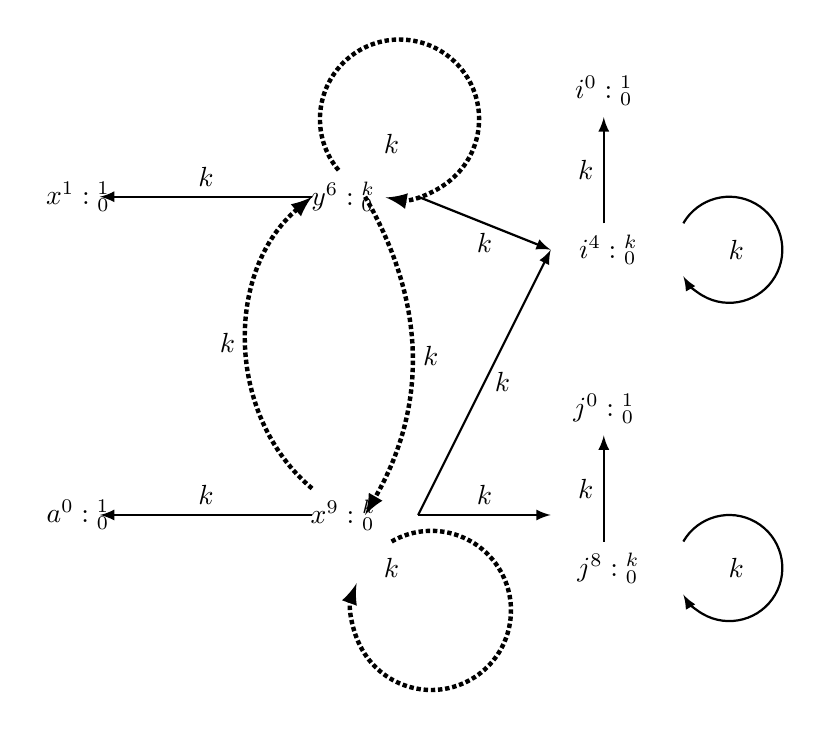
\begin{tikzpicture}[scale=\textwidth/18cm,samples=200]
      % Variables Initialization
      \draw[] (-5, 1) circle (0pt) node{{ $a^0: {}^1_{0}$}};
      \draw[] (-5, 7) circle (0pt) node{{ $x^1: {}^{1}_{0}$}};
      % Variables Inside the Loop
      \draw[] (0, 7) circle (0pt) node{{ $y^6: {}^{k}_{0}$}};
      \draw[] (0, 1) circle (0pt) node{{ $x^9: {}^{k}_{0}$}};
      % Counter Variables
      \draw[] (5, 9) circle (0pt) node {{$i^0: {}^{1}_{0}$}};
      \draw[] (5, 6) circle (0pt) node {{ $i^4: {}^{k}_{0}$}};
      \draw[] (5, 3) circle (0pt) node {{$j^0: {}^{1}_{0}$}};
      \draw[] (5, 0) circle (0pt) node {{ $j^8: {}^{k}_{0}$}};
      % Value Dependency Edges:
      \draw[ ultra thick, -latex, densely dotted,] (0, 7.5) arc (220:-100:1.5);
      \draw[] (1, 8) node [] {\highlight{$k$}};
      \draw[ thick, -latex] (5, 6.5)  -- node[left]{\highlight{{$k$}}}(5, 8.5) ;
      \draw[ thick, -latex] (5, 0.5)  -- node[left]{\highlight{{$k$}}}(5, 2.5) ;
      \draw[ ultra thick, -latex, densely dotted,] (1., 0.5) arc (120:-200:1.5);
      \draw[] (1, 0) node [] {\highlight{$k$}};
      % Value Dependency Edges on Initial Values:
      \draw[ thick, -latex,] (-0.5, 1)  -- node[above]{\highlight{{$k$}}}(-4.5, 1) ;
      \draw[ thick, -latex,] (-0.5, 7)  -- node[above]{\highlight{{$k$}}}(-4.5, 7) ;
      %
      \draw[ ultra thick, -latex, densely dotted,] (-0.5, 1.5)  to  [out=-220,in=220]  
      node[left]{\highlight{{$k$}}}(-0.5, 7);
      \draw[ ultra thick, -latex, densely dotted,]  (0.5, 7) to  [out=-60,in=60] 
      node[right]{\highlight{{$k$}}}(0.5, 1) ;
      % Control Dependency
      \draw[ thick, -latex, ] (6.5, 6.5) arc (150:-150:1);
      \draw[] (7.5, 6) node [] {\highlight{$k$}};
      \draw[ thick, -latex, ] (6.5, 0.5) arc (150:-150:1);
      \draw[] (7.5, 0) node [] {\highlight{$k$}};
      \draw[ thick,-latex] (1.5, 7)  -- node[below]{\highlight{{$k$}}}(4, 6) ;
      \draw[ thick,-latex] (1.5, 1)  -- node[right]{\highlight{{$k$}}}(4, 6) ;
      \draw[ thick,-latex] (1.5, 1)  -- node[above]{\highlight{{$k$}}}(4, 1) ;
   \end{tikzpicture}
   \caption{}
      \end{centering}
      \end{subfigure}
    }
     \caption{(a) Nested While Loop Example, (b) Execution-Based Dependency Graph, (c) The Static Program-Based Dependency graph.}
    \label{fig:alg_adaptsearch_nestedwhile}
    \vspace{-0.5cm}
    \end{figure}
    %
%     When we searched for a walk: $y^6 \to y^6$,
%   if we update the $\kw{flowcapacity}[y^6]$ as $k$ after visiting $y^6$ the second time 
%   on this walk,
%   % the walk $y^6 \to y^6$,
%   and continuously visit $x^9$,
%   then the $\kw{flowcapacity[k]}$ is 
%   updated as $\min(k, k^2)$.
%   So
%   %  which 
%   % restricting 
%   the visiting times of $x^9$ is restricted by $k$ on the walk $y^6 \to y^6 \to x^9$.
%   This restriction excludes the finite walk $y^6 \to y^6 \to x^9 \to x^9$ where $y^6$ and $x^9$ visited by $k^2$ times
%   in the computation. 
%   However, the finite walk $y^6 \to y^6 \to x^9 \to x^9$ where $y^6$ is visited $k$ times and $x^9$ $k^2$ times is 
%   a qualified walk, and exactly the longest walk we aim to find. So, by Non-updating the $\kw{flowcapacity}$ after 
%   visiting $y$ again, we guarantee that the visiting times og vertices on every searched walk will not be restricted by weights not on this walk,
%   i.e., the soundness.
%  \\
% In the last line of this dfs algorithm, line: 16, it returns the adaptivity heading out from its input vertex.
% \\
% By applying this deep first search strategy on every vertex on this SCC, 
% we compute the adaptivity of this SCC by taking the maximum 
% % adaptivity reaching every vertex on this SCC.
% value over every vertex.
% %
% The soundness is formally guaranteed in Lemma~\ref{lem:sound_adaptalg_scc} in Appendix~\ref{apdx:adaptalg_soundness}.
            % \begin{algorithm}
        % \caption{
        % {Refined Adaptivity on $\kw{SCC}$}
        % \label{alg:dfscycle_alg}
        % }
        % \begin{algorithmic}
        % \REQUIRE Weighted Directed Graph $G = (\vertxs, \edges, \weights, \qflag)$ with a start vertex $s$ and destination vertex $t$ .
        % \STATE  {\bf {$\kw{dfs_{refine}(G, c, visited)}$}:}  
        % \STATE {\bf init} 
        % \\
        % current node: $c$, 
        % % \\
        % % visited: List of length $|\vertxs|$, initialize with $\efalse$.
        % \\
        % results: $r$ : INT List of length $|\vertxs|$, initialize with $\qflag(v)$ for every vertex.
        % \\
        % $\kw{flowcapacity}$: INT List of length $|\vertxs|$, initialize MAXINT. 
        % \#\{For every vertex, recording the minimum weight when the walk reaching 
        % that vertex, inside a cycle\}
        % \\
        % querynum: INT List of length $|\vertxs|$, initialize with $\qflag(v)$ for every vertex. 
        % \#\{For every vertex, recording the query numbers when the walk reaching 
        % that vertex, inside a cycle\}
        % \\
        % % \STATE {\bf if} $c = s$:
        % % \STATE \qquad update the length of the longest path reaching this vertex
        % % $r[s] =  r[s] + $$\kw{flowcapacity}$[s] * querynum[s].
        % % \RETURN  \qquad $r[s]$.      
        % \STATE {\bf for}  all vertex $v$ having directed edge from $c$:
        % \STATE \qquad \qquad $\kw{flowcapacity}$[v] = min($\weights(v)$, $\kw{flowcapacity}$[c]);
        % \STATE \qquad \qquad querynum[v] = querynum[c] + $\qflag(v)$;
        % \STATE \qquad \qquad \#\{do not update the length of the longest walk reaching $v$ until the cycle is finished\}
        % \STATE \qquad \qquad $r[v] =  r[c] $;
        % \STATE \qquad {\bf if}  $v$ is unvisited:
        % \STATE \qquad \qquad \#\{mark $v$ as visited\} $\kw{visited}[v] = 1$;
        % \STATE \qquad \qquad $\kw{dfs_{refine}(G, v, visited)}$;
        % \STATE \qquad {\bf else}: \#\{There is a cycle finished\}
        % \STATE \qquad \qquad \#\{update the length of the longest path reaching this vertex\}
        % \STATE \qquad \qquad 
        %  $r[v] =  \max(r[v], r[c] + $$\kw{flowcapacity}$[v] * querynum[v]);
        %  \STATE \qquad \qquad \#\{Recover the $\kw{flowcapacity}$ and querynumber to previous state, for different loops\}
        %  \STATE \qquad \qquad $\kw{flowcapacity}$[v] = $\kw{flowcapacity}$[c];
        %  \STATE \qquad \qquad querynum[v] = querynum[c];
        % \RETURN  $r[c]$
        % \end{algorithmic}
        % \end{algorithm}
        % %
        \begin{algorithm}
          \caption{
          {Over-Approximated Adaptivity on SCC}
          \label{alg:overadp_alg}
          }
          \begin{algorithmic}[1]
          \REQUIRE $G = (\vertxs, \edges, \weights, \qflag)$ \#\{An Strong Connected Symbolic Weighted Directed Graph\}
          % with a start vertex $s$ and destination vertex $t$ .
          \STATE {\bf {$\kw{\pathsearch_{scc-naive}(G)}$}:}  
          \STATE {\bf init} 
          \\
          $\kw{r_{scc}}$: the Adaptivity of this SCC
          % \STATE  {\bf def} {$\kw{dfs_{naive}(G, c,visited)}$}: 
          % % \STATE {\bf init} 
          % % \\
          % % current node: $c$, 
          % % \\
          % % visited: List of length $|\vertxs|$, initialize with $\efalse$.
          % % \\
          % % \STATE {\bf if} $c = s$:
          % % \RETURN \qquad  $\weights(s)*\flag(s) $.
          % \STATE \qquad $r[c] = \weights(c)*\qflag(c) $
          % \STATE \qquad {\bf for}  all vertex $v$ having directed edge from $c$:
          % \STATE \qquad \qquad {\bf if}  $v$ is unvisited:
          % \STATE \qquad \qquad \qquad  \#\{mark $v$ as visited\} $\kw{visited}[v] = 1$;
          % \STATE \qquad \qquad \qquad $r[c] += \kw{dfs_{naive}(G, v, visited)}$;
          % \STATE \qquad {\bf else}: \#\{There is a cycle finished\}
          % \RETURN \qquad \qquad $\weights(v)*\flag(v) $.
          \STATE  {\bf for} every vertex $v$ in $\vertxs$:
          % \STATE  \qquad initialize \kw{visited} with $\efalse$.
          \STATE  \qquad $r_{scc} += \weights(v)*\qflag(v)$  
          \RETURN $r[c]$
          \end{algorithmic}
          \end{algorithm}
          %
\begin{thm}[Soundness of $\pathsearch$]
    \label{thm:sound_adaptalg}
    For every program $c$, given its \emph{Program-Based Dependency Graph} $\progG$,
     $$\pathsearch(\progG) \geq \progA(\progG).$$
\end{thm}
% \input{adaptalg_soundness.tex}
% % \paragraph{Variable Collection Algorithm, $\varCol$}
% % % The $\varCol$ algorithm shows how the labelled variables $\lvar$ are collected 
% % % (via the command ${\assign{x}{\expr}}$ or ${\assign{x}{\query(\qexpr)}}$) from the program ${c}$ in the first step.
% % % The algorithmic rules for $\varCol$ algorithm is defined in Figure~\ref{fig:var_col}. 
% % % It has the form: $\ag{\lvar; w; {c}}{ \lvar'; w'} $. 
% % % The input of $\varCol$ is the labelled variables $\lvar$ collected before the program ${c}$, a while map $w$ consistent with previous estimation, a program ${c}$. 
% % % The output of the algorithm is the updated labelled variables $\lvar'$, along with the updated while map $w$ for next steps' collecting.   
% % The $\varCol$ algorithm shows how the labelled variables $\lvar$ are collected 
% % (via the command ${\assign{x}{\expr}}$ or ${\assign{x}{\query(\qexpr)}}$) from the program ${c}$ in the first step, 
% % along with constructing the flag for each variable, i.e., $\flag$.
% % The algorithmic rules for $\varCol$ algorithm is defined in Figure~\ref{fig:var_col}. 
% % It has the form: 
% % {$\ag{\lvar; \flag; {c}}{ \lvar'; \flag'} $}. 
% % The input of $\varCol$ is a program ${c}$, 
% % the labelled variables $\lvar$ collected before the program ${c}$ 
% % as well as the flags $\flag$ for every corresponding variable .
% % The output of the algorithm is the updated labelled variables $\lvar'$ and flags $\flag'$ thorough the program ${c}$
% % %
% % % We have the algorithmic rules for $\varCol$ algorithm of the form: $\ag{\lvar; w; {c}}{\lvar';w'} $ as in Figure \ref{fig:var_col}. 
% % %
% % \begin{figure}
% % {
% % \begin{mathpar}
% % \inferrule
% % {
% % \empty
% % }
% % { \ag{\lvar ; \flag; {[\assign {x}{\expr}]^{l}}}
% % {\lvar ++ [{x}]; \flag++[0]}
% % }
% % ~\textbf{\varCol-asgn}
% % \and
% % \inferrule
% % {
% % }
% % { \ag{\lvar; \flag; [ \assign{{x}}{\query({\qexpr})}]^{l}}
% % {\lvar ++ [{x}]; \flag ++ [2]} 
% % }~\textbf{\varCol-query}
% % %
% % \and 
% % %
% % \inferrule
% % {
% % \ag{\lvar; [];  {c_1}}{\lvar_1; \flag_1}
% % \and 
% % \ag{\lvar_1; []; {c_2}}{ \lvar_2; \flag_2}
% % \and
% % \lvar_3 = \lvar_2 ++ \lvar'
% % \and
% % \flag_3 = \flag ++ ((\flag_1 ++ \flag_2) \uplus 1)
% % }
% % {
% % \ag{\lvar; \flag;
% % [\eif({\bexpr}, { c_1, c_2)}]^{l} }
% % {\lvar_3; \flag_3}
% % }~\textbf{\varCol-if}
% % %
% % %
% % %
% % \and 
% % %
% % \inferrule
% % {
% % \ag{\lvar; \flag {c_1}}{\lvar_1; \flag_1}
% % \and 
% % \ag{\lvar_1; \flag_1 ; {c_2}}{\lvar_2; \flag_2}
% % }
% % {
% % \ag{\lvar; \flag;
% % {(c_1 ; c_2)}}{\lvar_2 ; \flag_2}
% % }
% % ~\textbf{\varCol-seq}
% % \and 
% % %
% % %
% % {
% % \inferrule
% % {
% % { \ag{\lvar; [] ; {c}}
% % {\lvar'; \flag' }  }
% % \\
% % \lvar'' = \lvar'
% % \and 
% % \flag'' = \flag ++ (\flag' \uplus 1)
% % }
% % {
% % \ag{\lvar; \flag;  
% % \ewhile [{b}]^{l}
% % \edo  {c} }{\lvar''; \flag''}
% % }
% % ~\textbf{\varCol-while}
% % }
% % \end{mathpar}
% % }
% % \caption{The Algorithmic Rules of $\varCol$ }
% % \label{fig:var_col}
% % \end{figure}
% % %
% % %
% % The assignment commands are the source of variables $\varCol$ collecting, 
% % in the case $\textbf{\varCol-asgn}$ and $\textbf{\varCol-query}$, 
% % the output labelled variables are extended by ${x}$. 
% % \\
% % \todo{
% % When it comes to the $\eif \ldots \ethen \ldots \eelse$ command in the rule $\textbf{\varCol-if}$, variables assigned in the then branch ${c_1}$, as well as the variables assigned in the else branch ${c_2}$, and the new generated variables $\bar{{x}},\bar{{y}},\bar{{z}}$ in $ [ \bar{{x}}, \bar{{x_1}}, \bar{{x_2}}] ,[ \bar{{y}}, \bar{{y_1}}, \bar{{y_2}}],[ \bar{{z}}, \bar{{z_1}}, \bar{{z_2}}]$.
% % \\ 
% % The sequence command ${c_1;c_2}$ is standard by accumulating the predicted variables in the two commands ${c_1}$ and ${c_2}$ preserving their order. 
% % \\
% % The while command $\ewhile {\bexpr}, [{\bar{x}}] \ldots \edo {c}$ considers the newly generated variables by SSA transformation ${\bar{x}}$
% % as well and the newly labelled variables in its body ${c}$.
% % \\
% % %
% % Below we present the definition for a valid index, to have a clear understanding on the variable collecting algorithm:
% % }
% % %
% % %
% % \todo{
% % \begin{defn}[Valid Index (Remove?)]
% % Given an assigned variable list $\lvar$, $\lvar; \vDash ({c},i_1,i_2)$ iff 
% % $\lvar' = \lvar[0,\ldots, i_1-1], \lvar';{c} \to \lvar'' \land \lvar'' = \lvar[0, \ldots, i_2-1] $.  
% % \end{defn}}
% % %
% % %
% \todo{Data Dependency Analysis Algorithm Needed: (Possibly modify based on existing one, or a different one) get the more precise dependency information. 
% i.e., instead of dependency on all the over-approximated variables, 
% but dependency on only the variables assumed to be live.
% }
% \paragraph{Data Dependency Analysis Algorithm}
% %
% In this data flow matrix generating algorithm, we analyze the data flow information among all labelled variables $\lvar$ collected via the the $\varCol$ algorithm of length $N$.
% %
% We track the data flow relations between all these labelled variables. These informations are stored in a matrix $\Mtrix$, whose size is $N \times N$. 
% % We also track whether arbitrary variable is assigned with a query result in a vector $\flag$ with size $|\lvar|$. 
% %
% The algorithm to fill in the matrix is of the form: 
% {$\ad{\Gamma ; {c} ; \lvar}{\Mtrix}$}
% $\ad{\Gamma ; {c} ; i_1, i_2}{\Mtrix; \flag}$. 
% $\Gamma$ is a vector records the variables the current program ${c}$ depends on, the index $i_1$ is a pointer which refers to the position of the first new-generated variable in ${c}$ in the labelled variables $\lvar$, and $i_2$ points to the first new variable that is not in ${c}$ (if exists). 
% % %
% % %
% % {
% % \begin{defn}[Valid Gamma (Remove?)]
% % $\Gamma \vDash i_1$ iff $\forall i \geq i_1, \Gamma(i_1)=0 $.  
% % \end{defn}
% % }
% %%
% %
% % \framebox{$ {\Gamma} \vdash^{i_1, i_2}_{\Mtrix, \flag} ~ c $}
% % \begin{mathpar}
% % \inferrule
% % {\Mtrix = \lMtrix_i * ( \rMtrix_{{\expr},i} + \Gamma )
% % }
% % {
% %  \ad{\Gamma;[\assign {{x}}{{\expr}} ]^{l}; i }{\Mtrix; \flag_{0}; i+1 }
% % }
% % ~\textbf{\graphGen-asgn}
% % \and
% % {
% % \inferrule
% % {\Mtrix = \lMtrix_i * ( \rMtrix_{{\expr},i} + \Gamma )
% % \\
% % \flag = \lMtrix_i \and \flag(i) = 1
% % }
% % { 
% % \ad{\Gamma;[ \assign{{x}}{\query({\expr})} ]^{l} ; i }
% % {\Mtrix;\flag;i+1}
% % }~\textbf{\graphGen-query}}
% % %
% % \and 
% % %
% % {
% % \inferrule
% % {
% % {\ad{\Gamma + \rMtrix_{{\bexpr}, i_1}; {c_1} ; i_1 }{ \Mtrix_1;\flag_1;i_2 }}
% % \and 
% % {\ad{\Gamma + \rMtrix_{{\bexpr}, i_1};{c_2} ; i_2 }{ \Mtrix_2; \flag_2 ;i_3}}
% % \\
% % {\ad{\Gamma; [ \bar{{x}}, \bar{{x_1}}, \bar{{x_2}}]; i_3 }{ M_x; \flag_{\emptyset}; i_3+|\bar{{x}}| }}
% % %
% % \\
% % %
% % {\ad{\Gamma; [ \bar{{y}}, \bar{{y_1}}, \bar{{y_2}}]; i_3+|\bar{{x}}| }{ \Mtrix_y; \flag_{\emptyset}; i_3+|\bar{{x}}|+|\bar{{y}}| }}
% % %
% % \\
% % %
% % {\ad{\Gamma; [ \bar{{z}}, \bar{{z_1}}, \bar{{z_2}}]; i_3+|\bar{{x}}|+ |\bar{{y}}|}{ \Mtrix_y; \flag_{\emptyset}; i_3+|\bar{{x}}|+|\bar{{y}}| + |\bar{{z}}| }}
% % \\
% % {\Mtrix = (\Mtrix_1 + \Mtrix_2)+ \Mtrix_x+ \Mtrix_y + \Mtrix_z }
% % }
% % {
% % \ad{\Gamma ; \eif([{\bexpr}]^{l},[ \bar{{x}}, \bar{{x_1}},
% % \bar{{x_2}}] ,[ \bar{{y}}, \bar{{y_1}}, \bar{{y_2}}], 
% % [ \bar{{z}}, \bar{{z_1}}, \bar{{z_2}}],
% % { c_1, c_2)} ; i_1}{ \Mtrix ; \flag_1 \uplus \flag_2 \uplus 2  ; i_3+|\bar{x}|+|\bar{y}|+|\bar{z}| }
% % }
% % ~\textbf{\graphGen-if}
% % }
% % %
% % %
% % %
% % \and 
% % %
% % \inferrule
% % {
% % {\ad{\Gamma; {c_1} ; i_1 }{ \Mtrix_1 ; \flag_1; i_2 }  }
% % \and 
% % {
% % \ad{\Gamma;{c_2}; i_2}{ \Mtrix_2; \flag_2 ;i_3 }}
% % }
% % {
% % \ad{\Gamma ; ({c_1 ; c_2} ) ; i_1}{( \Mtrix_1 {;} \Mtrix_2) ; \flag_1 \uplus V_2 ; i_3  }
% % }
% % ~\textbf{\graphGen-seq}
% % %
% % \and 
% % %
% % \and 
% % %
% % { 
% % \inferrule
% % {
% % B= |{\bar{x}}| \and {A = |{c}|}
% % \\
% % {\ad{\Gamma;[\bar{{x}}, \bar{{x_1}}, \bar{{x_2}}]; i+ (B+A) }{ \Mtrix_{1};V_{1}; i+B+(B+A) }}
% % \\
% % {
% % \ad{\Gamma;{c} ; i+B+(B+A)  }{ \Mtrix_{2}; \flag_{2}; i+B+A+(B+A) }
% % }
% % \\
% % {
% % \ad{\Gamma ; [\bar{{x}}, \bar{{x_1}}, \bar{{x_2}}] ; i+(B+A) }{ \Mtrix; \flag ;i+(B+A)+B}
% % }
% % \\
% % { \Mtrix' = \Mtrix + ( \Mtrix_{1} + \Mtrix_{2}) }
% % \and
% % {
% % \flag' = \flag \uplus (( \flag_{1} \uplus \flag_{2}) \uplus 2)  }
% % }
% % {
% % \ad{\Gamma;
% % \ewhile ~ [ b ]^{l} ~ {n} ~
% % [\bar{{x}}, \bar{{x_1}}, \bar{{x_2}}] 
% % ~ \edo ~  c;
% % i }{ \Mtrix'; \flag' ;i+(B+A)+B }
% % }~\textbf{\graphGen-while}
% % }
% % \end{mathpar}
% {
% \framebox{$ \ad{\Gamma; c; \lvar_c}{\Mtrix}$}
% \begin{mathpar}
% \inferrule
% {
% {x}^l \in \lvar_c
% \and 
% \Mtrix = \lMtrix_i * ( \rMtrix_{{\expr}} + \Gamma )
% }
% {
% \ad{\Gamma; [\assign {{x}}{{\expr}} ]^{l}; \lvar_c}
% {\Mtrix}
% }
% ~\textbf{\graphGen-asgn}
% \and
% {
% \inferrule
% {
% {x}^l \in \lvar_c
% \and 
% \Mtrix = \lMtrix_i * ( \rMtrix_{{\expr}} + \Gamma )
% }
% { 
% \ad{\Gamma;[ \assign{{x}}{\query({\qexpr})} ]^{l} ; \lvar_c }
% {\Mtrix}
% }~\textbf{\graphGen-query}}
% %
% \and 
% %
% {
% \inferrule
% {
% {\ad{\Gamma + \rMtrix_{{\bexpr}}; {c_1} ; \lvar_c }{ \Mtrix_1}}
% \and 
% {\ad{\Gamma + \rMtrix_{{\bexpr}}; {c_2}; \lvar_c }{ \Mtrix_2}}
% \and
% {\Mtrix = (\Mtrix_1 + \Mtrix_2)}
% }
% {
% \ad{\Gamma ; \eif([{\bexpr}]^{l},{ c_1, c_2)}}
% { \Mtrix }
% }
% ~\textbf{\graphGen-if}
% }
% %
% %
% %
% \and 
% %
% \inferrule
% {
% {\ad{\Gamma; {c_1}; \lvar_c }{ \Mtrix_1}  }
% \and 
% {
% \ad{\Gamma;{c_2}; \lvar_c }{ \Mtrix_2}}
% }
% {
% \ad{\Gamma ; ({c_1 ; c_2} ); \lvar_c}
% {( \Mtrix_1 {;} \Mtrix_2) }
% }
% ~\textbf{\graphGen-seq}
% %
% \and 
% %
% \and 
% %
% { 
% \inferrule
% {
% {
% \ad{\Gamma + \rMtrix_{{\bexpr}};{c}; \lvar_c  }{ \Mtrix'}
% }
% }
% {
% \ad{\Gamma;
% \ewhile [ \sbexpr ]^{l} \edo  {c}; \lvar_c }{\Mtrix'}
% }~\textbf{\graphGen-while}
% }
% \end{mathpar}
% }
% %
% Below we define the valid data flow matrix, to have a clear understanding on the data flow generating algorithm:
% \begin{defn}[Valid Matrix]
% For a labelled variables $\lvar$, $\lvar \vDash (\Mtrix,\flag)$ iff the cardinality of $\lvar$ equals to the one of $\flag$, $|\lvar| = |\flag|$ 
% and the matrix $\Mtrix$ is of size $|\flag| \times |\flag|$.
% \end{defn}
% %
% \todo{Improvement if possible: Combining reachability bounds analysis into the static dependency analysis algorithm above, rather than adopting an external tool entirely.}
% %
% \paragraph{Reachability Bounds}
% Given a program $c$ with its labelled variables $\lvar$,
% we use the $\rb({x}, {c})$ algorithm, from paper \cite{10.1145/1806596.1806630}, to estimate the reachability bound for each variable ${x} \in \lvar$. 
% The input of $\rb$ is a program ${c}$ in SSA language and a variable ${x} $ from ${c}$.
% The output of $\rb({x}, {c})$ is an integer representing the reachability bound of ${x}$ in ${c}$.
% %

% %
% The following example programs ${c}2$ and ${c}3$ with while loop illustrate how the algorithm works.
% The collected labelled variables, $\lvar_{{c}2}$ and $\lvar_{{c}3}$,
% data flow matrix $\Mtrix_{{c}2}$ and  $\Mtrix_{{c}3}$
% and variable flags $\flag_{{c}2}$ and $\flag_{{c}3}$
% for program ${c}2$ and ${c}3$
% are presented in the right hand side.
%
% \[
% {{c}2 \triangleq
% \begin{array}{l}
% \left[{ x_1} \leftarrow \query(1)  \right]^1 ; 
% \\
% \left[{i_1} \leftarrow 0 \right]^2 ; 
% \\
% \ewhile
% ~ [{i_1} < 2]^3
% 	\\
% ~{[ x_3,x_1 ,x_2 ], [i_3, i_1, i_2] }
% ~ \edo 
% \\
% ~ \Big( 
% \left[{y}_1 \leftarrow \query(2) \right]^4;
% \\
% \left[{x_2 \leftarrow y_1  + x_3 } \right]^5;
% \\
% \left[{i_2 \leftarrow 1  + i_3 } \right]^6
% \Big) ; 
% \\
% \left[ {\assign{z_1}{x_3}} + 2  \right]^{7}
% \end{array}
% ,
% ~~~~
% \lvar_{{c}2} = \left [ \begin{matrix}
% {x}_1 \\
% {x}_3 \\
% {y}_1 \\
% {x}_2 \\
% {z}_1 \\
% {i}_1 \\
% {i}_2 \\
% {i}_3 
% \end{matrix} \right ]
% % \Mtrix =  \left[ \begin{matrix}
% %  & (x_1)  & (y_1) & (x_2) & (x_3) &  (z_1) & i_1 & i_2 & i_3\\
% % (x_1) & 0 & 0 & 0 & 0 & 0 & 0 & 0 & 0 \\
% % (y_1) & 0 & 0 & 0 & 0 & 0 & 1 & 1 & 1 \\
% % (x_2) & 0 & 1 & 0 & 1 & 0 & 1 & 1 & 1 \\
% % (x_3) & 1 & 0  & 1& 0 & 0 & 1 & 1 & 1 \\
% % (z_1) & 0 & 0 & 0 & 1 & 0 & 0 & 0 & 0 \\
% % (i_1) & 0 & 0 & 0 & 0 & 0 & 0 & 0 & 0 \\
% % (i_2) & 0 & 1 & 0 & 1 & 0 & 1 & 0 & 1 \\
% % (i_3) & 1 & 0  & 1& 0 & 0 & 1 & 1 & 1 \\
% % \end{matrix} \right]
% ,
% ~~~~~~
% \Mtrix_{{c}2} =  \left[ \begin{matrix}
% 0 & 0 & 0 & 0 & 0 & 0 & 0 & 0 \\
% 0 & 0 & 0 & 0 & 0 & 1 & 1 & 1 \\
% 0 & 1 & 0 & 1 & 0 & 1 & 1 & 1 \\
% 1 & 0  & 1& 0 & 0 & 1 & 1 & 1 \\
% 0 & 0 & 0 & 1 & 0 & 0 & 0 & 0 \\
% 0 & 0 & 0 & 0 & 0 & 0 & 0 & 0 \\
% 0 & 1 & 0 & 1 & 0 & 1 & 0 & 1 \\
% 1 & 0  & 1& 0 & 0 & 1 & 1 & 1 \\
% \end{matrix} \right]
% ,
% ~~~~
% \flag_{{c}2} = \left [ \begin{matrix}
% 1 \\
% 2 \\
% 1 \\
% 2 \\
% 0 \\
% 0 \\
% 2 \\
% 1 
% \end{matrix} \right ]
% }
% \]
% %
% %
% \[
% {{{c}3}  \triangleq
% \begin{array}{l}
% \left[{ x}_1 \leftarrow \query(1)  \right]^1 ;
% \\
% \left[{i_1} \leftarrow 1 \right]^2 ; 
% \\
% \ewhile ~ [i < 0]^{3} ,
% \\
% ~{[ x_3,x_1 ,x_2 ], [i_3, i_1, i_2] }
% ~ \edo
% \\
% ~ \Big( 
% \left[{ y_1} \leftarrow \query(2) \right]^3; \\
% \left[{x_2 \leftarrow y_1  + x_3 } \right]^5
% \Big) ; \\
% \left[ {\assign{z_1}{x_3}} + 2  \right]^{6}
% \end{array},
% ~~~~~~
% \lvar_{{c}3} = \left [ \begin{matrix}
% {x}_1 \\
% {i}_1 \\
% {x}_3 \\
% {i}_3 \\
% {z}_1 \\
% \end{matrix} \right ]
% ,~~~~~~
% \Mtrix_{{c}3}  =  \left[ \begin{matrix}
% 0 & 0 & 0 & 0 & 0 \\
% 0 & 0 & 0 & 0 & 0 \\
% 1 & 0 & 0 & 0 & 0 \\
% 0 & 1 & 0 & 0 & 0 \\
% 0 & 0 & 1 & 0 & 0 \\
% \end{matrix} \right]
% ,~~~~~~
% \flag_{{c}3} = \left [ \begin{matrix}
% 1 \\
% 0 \\
% 2 \\
% 2 \\
% 0 \\
% \end{matrix} \right ]
% }
% \]
% %
% We can now look at the if statement.
% \[ 
% %
% {c}4 \triangleq
% \begin{array}{l}
% 	\left[ {x}_1 \leftarrow \query(1) \right]^1; 
% 	\\
% 	\left[{y}_1 \leftarrow \query(2) \right]^2 ; 
% 	\\
% \eif \;( { x_1 + y_1 == 5} )^3,  \\
% {[ x_4,x_2,x_3 ],[] ,[y_3,y_1,y_2 ]} 
% \\
% \mathsf{then} ~ \left[ 
% {x}_2 \leftarrow \query(3) \right]^4 
% \\
% \mathsf{else} ~ \left[ 
% {x}_3 \leftarrow \query(4) \right]^5 ; 
% \\
% {y}_2 \leftarrow 2 ) \\
% \left[ { z_1 \leftarrow x_4 +y_3 }\right]^6
% \end{array},
% % \]
% % \[
% ~~~~~~
% \lvar_{{c}4} =  \left[ \begin{matrix}
% {x}_1 \\
% {y}_1 \\
% {x}_2 \\
% {x}_3 \\
% {y}_2 \\
% {x}_4 \\
% {y}_3 \\
% {z}_1 \\
% \end{matrix} \right], 
% ~~~~~ 
% \Mtrix_{{c}4} =  \left[ \begin{matrix}
% 0 & 0 & 0 & 0 & 0 & 0 & 0 & 0 \\
% 0 & 0 & 0 & 0 & 0 & 0 & 0 & 0 \\
% 0 & 0 & 0 & 0 & 0 & 0 & 0 & 0 \\
% 0 & 0 & 0 & 0 & 0 & 0 & 0 & 0 \\
% 0 & 0 & 0 & 0 & 0 & 0 & 0 & 0 \\
% 0 & 0 & 1 & 1 & 0 & 0 & 0 & 0 \\
% 0 & 1 & 0 & 0 & 1 & 0 & 0 & 0 \\
% 0 & 0 & 0 & 0 & 0 & 1 & 1 & 0 \\
% \end{matrix} \right], 
% ~~~~~ 
% \flag_{{c}4} = \left [ \begin{matrix}
% 1 \\
% 1 \\
% 1 \\
% 1 \\
% 0 \\
% 0 \\
% 0 \\
% 0 \\
% \end{matrix} \right ]
% \]
%
%
%
%


% By specifying the departure and destination vertices $s$ and $t$, the $\pathssearch(\progG, s, t)$ algorithm will 
% give the number of query vertices on a finite walk from $s$ to $t$, which contains the maximum number of query vertices.
% The pseudo-code of $\pathssearch(\progG, s, t)$ algorithm is defined in the Algorithm \ref{alg:adpt_alg}.
% %
% \begin{algorithm}
% \caption{
% {Walk Search Algorithm ($\pathssearch$)}
% \label{alg:adpt_alg}
% }
% \begin{algorithmic}
% \REQUIRE Weighted Directed Graph $G = (\vertxs, \edges, \weights, \flag)$ with a start vertex $s$ and destination vertex $t$ .
% \STATE  {\bf {bfs $(G, s, t)$}:}  
% \STATE \qquad {\bf init} 
% current node: $c = s$, 
% queue: $q = [c]$, 
% vector recoding if the vertex is visited: 
% visited$ = [0]*|\vertxs|$,
% result: $r$
% \STATE \qquad {\bf while} $q$ isn't empty:
% \STATE \qquad \qquad take the vertex from beginning $c= q.pop()$
% \STATE \qquad \qquad mark $c$ as visited, visited $[c] = 1$
% \STATE \qquad \qquad curr$\kw{flowcapacity}$ = min($\weights$(c), curr$\kw{flowcapacity}$).
% \STATE \qquad \qquad put all unvisited vertex $v$ having directed edge from c into $q$. 
% \STATE \qquad \qquad if $v$ is visited, then there is a circle in the graph, we update the result $r = r + $curr$\kw{flowcapacity}$
% \RETURN $r$
% \end{algorithmic}
% \end{algorithm}
%
%
% \subsection{\todo{Soundness of the \THESYSTEM}}

% {
% 	\begin{thm}[Soundness of the \THESYSTEM].
% 	Given a program ${c}$, we have:
% 	%
% 	\[
% 	\progA({c}) \geq A({c}).
% 	\]
% 	\end{thm}
% }
% {
% \begin{proof}
% Given a program ${c}$, 
% we construct its program-based graph $\progG({c}) = (\vertxs, \edges, \weights, \qflag)$
% by Definition~\ref{def:prog-based_graph}
% According to the Definition \ref{def:prog_adapt}, we have:
% %
% \[
% 	\progA({c}) 
% 	:= \max\left\{ \qlen(k)\ \mid \  k\in \walks(\progG({c}))\right \}.
% \]
% %
% According to the Definition \ref{def:trace-based_adapt}, we have the trace-based adaptivity as follows:
% $$
% A({c}) = \max \big 
% \{ \len(p) \mid {m} \in \mathcal{SM},D \in \dbdom ,p \in \paths(\traceG({c}, \text{D}, {m}) \big \} 
% $$
% %
% Then, we need to show:
% \[
% \max \big 
% \{ \len(p) \mid {m} \in \mathcal{SM},D \in \dbdom ,p \in \paths(\traceG({c}, \text{D}, {m}) \big \} 
% \leq
% \max\left\{ \qlen(k) \ \mid \  k\in \walks(\progG({c}))\right \}
% \]
% %
% It is sufficient to show that:
% \[
% 	\forall p, {m}, D, ~ s.t., ~ p \in \paths(\traceG({c}, \text{D}, {m}),
% 	\exists k \in \walks(\progG({c})) \land 
% 	\len(p) \leq \qlen(k)
% \]
% %
% Taking an arbitrary starting memory $m$ and an arbitrary underlying database $D$,
% we construct a trace-based graph $\traceG({c}, \text{D}, {m}) = (\vertxs, \edges)$ by the definition \ref{def:trace-based_graph}.
% %
% \\
% %
% Let $\midG({c},{m},\text{D}) = \{\midV, \midE, \midF\}$ be the intermediate graph by Definition~\ref{def:midgraph}.
% \\
% By Lemma~\ref{lem:bie_trace_to_mid}, we know:
% \[
% 	\forall p, {m}, D, ~ s.t., ~ p \in \paths(\traceG({c}, \text{D}, {m}),
% 	\exists p' \in \paths(\midG({c},{m},\text{D})) \land 
% 	\len(p) = \len_q(p')
% \]
% %
% Then it is sufficient to show that:
% %
% \[
% 	\forall p, {m}, D, ~ s.t., ~ p \in \paths(\midG({c}, \text{D}, {m}),
% 	\exists k \in \walks(\progG({c})) \land 
% 	\qlen(p) \leq \qlen(k)
% \]
% %
% We prove a stronger statement instead:
% \[
% 	\forall p, {m}, D, ~ s.t., ~ p \in \paths(\midG({c}, \text{D}, {m}),
% 	\exists k \in \walks(\progG({c})) \land 
% 	\qlen(p) = \qlen(k)	
% \]
% %
% %
% By Lemma~\ref{lem:sujv_mid_to_prog}, let $g$ be the surjective function $g: \progV \to \midV$ s.t.:
% %
% $$
% \forall \av \in \midV. ~ \progF(f(\av)) = \midF(\av) 
% \land |\kw{image}(f(\av))| \leq W(f(\av)).
% $$
% %
% %
% % \item(1) $\len(p_{\av_1 \to \av_2}) = \len(k_{f(\av_1) \to f(\av_2)})$
% % %
% % \item(2) $\forall \av \in p_{\av_1 \to \av_2}. ~ f(\av) \in k_{f(\av_1) \to f(\av_2)}$
% % %
% % \item(3) $\forall \av \in p_{\av_1 \to \av_2}. ~ 
% % \kw{image}(f(\av)) \cap {p_{\av_1 \to \av_2}}| = \# \{f(\av) \mid f(\av) \in k_{f(\av_1) \to f(\av_2)}\}$
% %
% Let ${m}$ and $D$ be an arbitrary memory and database $D$,
% taking an arbitrary path $p_{\av_1 \to \av_n} \in \paths(\midG({c}, \text{D}, {m})$ with:
% %
% \item Edge sequence: $(e, \ldots, e_{n-1})$
% %
% \item Vertices sequence: $(\av_1, \ldots, \av_n)$.
% \\
% By Lemma~\ref{lem:sujpathwalk_mid_to_prog}, let $h: \paths(\midG({c}, \text{D}, {m})) \to \walks(\progG({c}))$ be the surjective function satisfies:
% %
% \[
% 	\forall p_{\av_1 \to \av_n} \in \paths(\midG({c}, \text{D}, {m}))
% 	\text{ with }
% 	\left\{
% 	\begin{array}{ll}
% 	\mbox{edge sequence:} & (e, \ldots, e_{n-1})
% 	\\ 
% 	\mbox{vertices sequence:} & (\av_1, \ldots, \av_n)
% 	\end{array}
% 	\right.
% \]
% %
% \[
% 	\exists k_{f(\av_1) \to f(\av_n)} \in \walks(\progG({c}))
% 	\text{ with }
% 	\left\{
% 	\begin{array}{ll}
% 	\mbox{edge sequence:} & (g(e), \ldots, g(e_{n-1}) 
% 	\\ 
% 	\mbox{vertices sequence:} & (f(\av_1), \ldots, f(\av_{n}))
% 	\end{array}
% 	\right.
% \]
% %
% We have the walk:
% $k_{f(\av_1) \to f(\av_n)} \in \walks(\progG({c}))$ with:
% %
% \item Edges sequence: $(g(e), \ldots, g(e_{n-1}) $
% %
% \item Vertices sequence: $(f(\av_1), \ldots, f(\av_{n}))$.
% \\
% It is sufficient to show 
% %
% \[
% 	\qlen(p_{\av_1 \to \av_n}) = \qlen(k_{f(\av_1) \to f(\av_n)})
% \]
% %
% Unfold the definition of $\qlen$, it is suffice to show:
% \[
% \len \big( \av \mid \av \in (\av_1, \ldots, \av_n) \land \midF(\av) = 2 \big) 
% = \len \big(f(\av) \mid f(\av) \in (f(\av_1), \ldots, f(\av_{n})) \land \progF(f(\av)\big) = 2)	
% ~ (a)
% \]
% %
% By Lemma~\ref{lem:sujv_mid_to_prog}, we know:
% %
% \[
% 	\forall \av \in \midV. ~ \midF(\av) = \progF(f(\av)) ~(b)
% \]
% By rewriting $(b)$ in $(a)$, we have this case proved.
% %
% \\
% \todo{
% \begin{defn}[Intermediate Graph $\midG$].
% 	\label{def:midgraph}
% 	\\
% 	$\mathcal{AV}$ : Annotated Variables based on program execution
% 	\\
% 	Given a program ${c}$ with its labelled variables $\lvar$ of length $N$,
% 	a database $D$, a starting memory ${m}$,
% 	s.t., $\Gamma \vdash_{\Mtrix_c, \flag_c} {c}$,
% 	the intermediate graph 
% 	$\midG({c},{m},\text{D}) = (\vertxs, \edges, \flag)$ is defined as:%
% \[
% \begin{array}{rlcl}
% 	\text{Vertices} &
% 	\vertxs & := & \left\{ 
% 	\av \in \mathcal{AV} \middle\vert
% 	\exists {m'},  w', \qtrace, \vtrace.  ~ s.t., ~  
% 	\config{{m} ,{c}, [], [], []}  \to^{*}  \config{{m'} , \eskip, \qtrace, \vtrace, w' }
% 	\land \av \in \vtrace
% 	\right\}
% 	\\
% 	\text{Directed Edges} &
% 	\edges & := & 
% 	\left\{ 
% 	(\av, \av') \in \mathcal{AV} \times \mathcal{AV} 
% 	~ \middle\vert ~
% 	\flowsto(\av, \av', {c},{m},D) 
% 	\right\}
% 	\\
% 	\text{Flags} &
% 	\flag & := & 
% 	\big\{ (\av, n)  \in \vertxs \times \{0, 1, 2\} 
% 	\mid 
% 	(\pi_1(\av) = \lvar(i) \land n = \flag_c(i)); ~
% 	i = 1, \ldots, N
% 	\big\}
% \end{array}
% \]
% \end{defn}
% }
% %
% \\
% \todo{
% 	\begin{lem}[$\vardep$ is Transitive].
% 	\label{lem:vardep_trans}
% 	\\
% 	Given a program ${c}$, with a starting memory ${m}$ and a hidden database $D$, s.t., 
% 	$\config{{m}, {c}, [], [], []} \rightarrow^{*} \config{{m}', \eskip, \qtrace, \vtrace, w} $.
% 	Then, $\forall \av_1, \av_2, \av_3 \in \vtrace$:
% \[
% 	\Big(\vardep(\av_1, \av_2, {c}, {m}, D) \land 
% 	\vardep(\av_2, \av_3, {c}, {m}, D) \Big)
% 	\implies
% 	\vardep(\av_1, \av_3, {c}, {m}, D)
% \]
% 	\end{lem}
% 	\begin{subproof}[of Lemma~\ref{lem:vardep_trans}]
% 	Proof by unfolding and rewriting the Definition~\ref{def:var_dep}.
% 	\end{subproof}
% }
% \\
% %
% \todo{
% 	\begin{lem}[$\flowsto$ is Transitive ??].
% 	\label{lem:flowsto_trans}
% 	\\
% 	Given a program ${c}$ with its labelled variables $\lvar$ of length $N$. 
% 	Then $\forall x_1, x_2, x_3 \in \lvar$
% \[
% 	\Big(\flowsto(x_1, x_2) \land \flowsto(x_2, x_3) \Big)
% 	\implies
% 	\flowsto(x_1, x_3)
% \]
% 	\end{lem}
% 	\begin{subproof}[of Lemma~\ref{lem:flowsto_trans}]
% 	Proof by unfolding the Definition~\ref{def:flowsto}.
% 	\end{subproof}
% }
% \\
% %
% \todo{
% 	\begin{lem}[$\qdep$ Implies $\vardep$].
% 	\label{lem:querydep_vardep}
% 	\\
% 	Given a program ${c}$, with a starting memory ${m}$ and a hidden database $D$, s.t., 
% 	$\config{{m}, {c}, [], [], []} \rightarrow^{*} \config{{m}', \eskip, \qtrace, \vtrace, w} $.
% 	Then, $\forall \av_1, \av_2 \in \qtrace$
% \[
% 	\qdep(\av_1, \av_2, {c}, {m}, D) \implies 
% 	\vardep(\pi_2(\av_1), \pi_2(\av_2), {c}, {m}, D)
% \]
% 	\end{lem}
% 	\begin{subproof}[of Lemma~\ref{lem:querydep_vardep}]
% 	Proof by unfolding the Definition~\ref{def:var_dep} and Definition~\ref{def:query_dep}.
% 	\end{subproof}
% }
% \\
% %
% \todo{
% 	\begin{lem}[$\vardep$ Implies \flowsto].
% 	\label{lem:vardep_flows}
% 	\\
% 	Given a program ${c}$, with a starting memory ${m}$ and a hidden database $D$, s.t., 
% 	$\config{{m}, {c}, [], [], []} \rightarrow^{*} \config{{m}', \eskip, \qtrace, \vtrace, w} $.
% 	Then, $\forall \av_1, \av_2 \in \vtrace$
% \[
% 	\vardep(\av_1, \av_2, {c}, {m}, D) \implies 
% 	\flowsto(\pi_1(\av_1), \pi_1(\av_2))
% \]
% 	\end{lem}
% 	\begin{subproof}[of Lemma~\ref{lem:querydep_vardep}]
% 	Proof by showing contradiction based on the Definition~\ref{def:var_dep} and Definition~\ref{def:flowsto}.
% 	Let $\av_1, \av_2 \in \vtrace$ be 2 arbitrary annotated variables in the variable trace $\vtrace$,
% 	s.t., $\vardep(\av_1, \av_2, {c}, {m}, D)$.
% 	\\
% 	Unfolding the $\vardep$ definition, we have:	
% 	\end{subproof}
% }
% \\
% %
% \todo{
% 	\begin{lem}[Injective Mapping of vertices from $\traceG$ to $\midG$].
% 	\label{lem:injv_trace_to_mid}
% 	\\
% 	$\traceG({c}) = \{\traceV, \traceE\}$
% 	\\
% 	$\midG({c},{m},\text{D}) = \{\midV, \midE, \midF\}$
% \[
% 	\exists ~ \kw{injective} ~ f: \mathcal{AQ} \to \mathcal{AV}. 
% 	~ \forall \av \in \traceV. ~ 
% 	f(\av) \in \midV \land \midF(f(\av)) = 2
% \]
% 	\end{lem}
% \begin{subproof}
% Proving by Definition~\ref{def:midgraph} and Definition~\ref{def:prog_adapt}.
% \end{subproof}
% }
% \\
% \todo{
% 	\begin{lem}[One-on-One Mapping from $\edges$ of $\traceG$ to $\paths(\midG)$].
% 	\label{lem:bie_trace_to_mid}
% 	\\
% 	$\traceG({c}) = \{\traceV, \traceE\}$
% 	\\
% 	$\midG({c},{m},\text{D}) = \{\midV, \midE, \midF\}$
% 	\\
% 	An injective function $ f: \traceV \to \midV$ s.t.,
% 	$\forall \av \in \traceV. ~ \midF(f(\av)) = 2$ 
% \[
% 	\forall e = (\av_1, \av_2) \in \traceE. ~ 
% 	\exists p_{f(\av_1) \to f(\av_2)} \in \paths(\midG({c}, \text{D}, {m}))
% \]
% 	\end{lem}
% \begin{subproof}
% Proving by Lemma~\ref{lem:injv_trace_to_mid} and Definition~\ref{def:midgraph} and acyclic property of $\traceG$ and $\midG$.
% \end{subproof}
% }
% \\
% \todo{
% 	\begin{lem}[Surjective Mapping of Vertices from $\midG$ to $\progG$].
% 	\label{lem:sujv_mid_to_prog}
% 	\\
% 	$\midG({c},{m},\text{D}) = \{\midV, \midE, \midF\}$
% 	\\
% 	$\progG({c}) = \{\progV, \progE, \progF, \progW\}$
% 	\\
% 	$\exists ~ \kw{surjective} ~ f: \mathcal{AV} \to \mathcal{SVAR}.$
% 	%
% \[
% 	\forall \av \in \midV. ~ 
% 	f(\av) \in \progV \land \progF(f(\av)) = \midF(\av) \land
% 	|\kw{image}(f(\av))| \leq W(f(\av))
% \]
% \end{lem}
% \begin{subproof}
% Proving by Definition~\ref{def:midgraph}.
% \end{subproof}
% }
% \\
% \todo{
% 	\begin{lem}[Surjective Mapping from $\edges$ of $\midG)$ to $\edges$ of $\progG$].
% 	\label{lem:suje_mid_to_prog}
% 	\\
% 	$\midG({c},{m},\text{D}) = \{\midV, \midE, \midF\}$
% 	\\
% 	$\progG({c}) = \{\progV, \progE, \progF, \progW\}$
% 	\\
% 	A surjective function $f: \progV \to \midV$ s.t.,
% 	$\forall \av \in \midV. ~ \progF(f(\av)) = \midF(\av) \land |\kw{image}(f(\av))| \leq W(f(\av))$
% 	%
% \[
% 	\exists ~ \kw{surjective} ~ g: \midE \to \progE. ~
% 	\forall e_{mid} = (\av_1, \av_2) \in \midE. 
% 	\exists e_{prog} = ({f(\av_1), f(\av_2)}) \in \progE
% \]
% \end{lem}
% \begin{subproof}
% Proving by Lemma~\ref{lem:sujv_mid_to_prog}.
% \end{subproof}
% }
% \\
% \todo{
% 	\begin{lem}[Surjective Mapping from $\paths(\midG)$ to $\walks(\progG)$].
% 	\label{lem:sujpathwalk_mid_to_prog}
% 	\\
% 	$\midG({c},{m},\text{D}) = \{\midV, \midE, \midF\}$
% 	\\
% 	$\progG({c}) = \{\progV, \progE, \progF, \progW\}$
% 	\\
% 	A surjective function $f: \progV \to \midV$ s.t.,
% 	$\forall \av \in \midV. ~ \progF(f(\av)) = \midF(\av) \land |\kw{image}(f(\av))| \leq W(f(\av))$
% 	\\
% 	A surjective function $g: \midE \to \progE$ s.t.,
% 	$\forall e_{mid} = (\av_1, \av_2) \in \midE. 
% 	\exists e_{prog} = ({f(\av_1) \to f(\av_2)}) \in \progE$
% 	\\
% 	$\exists ~ \kw{surjective} ~ h: \paths(\midG({c},{m},\text{D})) \to \walks(\progG({c}))$ s.t.:
% 	%
% \[
% 	\forall p_{\av_1 \to \av_2} \in \paths(\midG({c},{m},\text{D}))
% 	\text{ with }
% 	\left\{
% 	\begin{array}{ll}
% 	\mbox{edge sequence:} & (e, \ldots, e_{n-1})
% 	\\ 
% 	\mbox{vertices sequence:} & (\av_1, \ldots, \av_n)
% 	\end{array}
% 	\right.
% \]
% \[
% 	\exists k_{f(\av_1) \to f(\av_2)} \in \walks(\progG({c}))
% 	\text{ with }
% 	\left\{
% 	\begin{array}{ll}
% 	\mbox{edge sequence:} & (g(e), \ldots, g(e_{n-1}) 
% 	\\ 
% 	\mbox{vertices sequence:} & (f(\av_1), \ldots, f(\av_{n}))
% 	\end{array}
% 	\right.
% \]
% % \item $(e, \ldots, e_{n-1})$, $(\av_1, \ldots, \av_n)$ are the edges sequence and vertices sequence of $p_{\av_1 \to \av_2}$.
% % then, 
% %  $\len(p_{\av_1 \to \av_2}) = \len(k_{f(\av_1) \to f(\av_2)})$
% % %
% % \item $\forall \av \in p_{\av_1 \to \av_2}. ~ f(\av) \in k_{f(\av_1) \to f(\av_2)}$
% % %
% % \item $\forall \av \in p_{\av_1 \to \av_2}. ~ 
% % \kw{image}(f(\av)) \cap {p_{\av_1 \to \av_2}}| = \# \{f(\av) \mid f(\av) \in k_{f(\av_1) \to f(\av_2)}\}
% % $
% \end{lem}
% %
% \begin{subproof}
% Proving by induction on the length of $l = p_{\av_1 \to \av_2} \in \paths(\midG({c},{m},\text{D}))$, and Lemma~\ref{lem:suje_mid_to_prog} and Lemma~\ref{lem:sujv_mid_to_prog}.
% \caseL{ $l = 1$: }
% \caseL{ $l = l' + 1$, $l' \geq 1$: }
% \end{subproof}
% }
% \end{proof}
% %

% %
% }
